%%%%%%%%%%%%%%%%%%%%%%%%%%%%%%% beamer %%%%%%%%%%%%%%%%%%%%%%%%%%%%%%%%%%%%%%%%%%%%%%%%%
% To run - pdflatex filename.tex
%      acroread filename.pdf
%%%%%%%%%%%%%%%%%%%%%%%%%%%%%%%%%%%%%%%%%%%%%%%%%%%%%%%%%%%%%%%%%%%%%%%%%%%%%%%%%%%%%%%%

\documentclass[compress,oilve]{beamer}
\mode<presentation>

\usetheme[]{CambridgeUS}
% other themes: AnnArbor, Antibes, Bergen, Berkeley, Berlin, Boadilla, boxes, CambridgeUS, Copenhagen, Darmstadt, default, Dresden, Frankfurt, Goettingen,
% Hannover, Ilmenau, JuanLesPins, Luebeck, Madrid, Maloe, Marburg, Montpellier, PaloAlto, Pittsburg, Rochester, Singapore, Szeged, classic

\usecolortheme{beaver}
% color themes: albatross, beaver, beetle, crane, default, dolphin,  fly, lily, orchid, rose, seagull, seahorse, sidebartab, whale, wolverine

\usefonttheme{professionalfonts}
% font themes: default, professionalfonts, serif, structurebold, structureitalicserif, structuresmallcapsserif


\hypersetup{pdfpagemode=FullScreen} % makes your presentation go automatically to full screen

% define your own colors:
\definecolor{Red}{rgb}{1,0,0}
\definecolor{Blue}{rgb}{0,0,1}
\definecolor{Green}{rgb}{0,1,0}
\definecolor{magenta}{rgb}{1,0,.6}
\definecolor{lightblue}{rgb}{0,.5,1}
\definecolor{lightpurple}{rgb}{0.8, 0.6, 0.9}
\definecolor{gold}{rgb}{.6,.5,0}
\definecolor{orange}{rgb}{1,0.4,0}
\definecolor{hotpink}{rgb}{1,0,0.5}
\definecolor{newcolor2}{rgb}{.5,.3,.5}
\definecolor{newcolor}{rgb}{0,.3,1}
\definecolor{newcolor3}{rgb}{1,0,.35}
\definecolor{darkgreen1}{rgb}{0, .35, 0}
\definecolor{darkgreen}{rgb}{0, .6, 0}
\definecolor{darkred}{rgb}{.75,0,0}
\definecolor{skyblue}{HTML}{75bbfd}

\definecolor{olive}{cmyk}{0.64,0,0.95,0.4}
\definecolor{purpleish}{cmyk}{0.75,0.75,0,0}

% can also choose different themes for the "inside" and "outside"

% \usepackage{beamerinnertheme_______}
% inner themes include circles, default, inmargin, rectangles, rounded

% \usepackage{beamerouterthemesmoothbars}
% outer themes include default, infolines, miniframes, shadow, sidebar, smoothbars, smoothtree, split, tree


\useoutertheme[subsection=true, height=40pt]{smoothbars}

% to have the same footer on all slides
%\setbeamertemplate{footline}[text line]{STUFF HERE!}
\setbeamertemplate{footline}[text line]{} % makes the footer EMPTY
% include packages
%

%show the page numbers in footnote
%\addtobeamertemplate{navigation symbols}{}{%
%	\usebeamerfont{footline}%
%	\usebeamercolor[fg]{footline}%
%	\hspace{1em}%
%	\insertframenumber/\inserttotalframenumber
%}

\setbeamercolor{footline}{fg=purpleish}
\setbeamerfont{footline}{series=\bfseries}

%add color to curent subsection
\setbeamertemplate{section in head/foot}{\hfill\tikz\node[rectangle, fill=darkred, rounded corners=1pt,inner sep=1pt,] {\textcolor{white}{\insertsectionhead}};}
\setbeamertemplate{section in head/foot shaded}{\textcolor{darkred}{\hfill\insertsectionhead}}

% Remove bullet of subsections
\setbeamertemplate{headline}
{%
	\begin{beamercolorbox}{section in head/foot}
		\insertsectionnavigationhorizontal{\textwidth}{}{}
	\end{beamercolorbox}%
}


% modify headlline, specially headline size
\setbeamertemplate{headline}{%
	\leavevmode%
	\hbox{%
		\begin{beamercolorbox}[wd=\paperwidth,ht=3.5ex,dp=1.125ex]{palette quaternary}%
			\insertsectionnavigationhorizontal{\paperwidth}{}{\hskip0pt plus1filll}
		\end{beamercolorbox}%
	}
}

\setbeamertemplate{footline}{%
	\leavevmode%
	\hbox{\begin{beamercolorbox}[wd=.5\paperwidth,ht=2.5ex,dp=1.125ex,leftskip=.3cm plus1fill,rightskip=.3cm]{author in head/foot}%
			\usebeamerfont{author in head/foot}\insertshortauthor ~ \insertshortinstitute
		\end{beamercolorbox}%
		\begin{beamercolorbox}[wd=.5\paperwidth,ht=2.5ex,dp=1.125ex,leftskip=.3cm,rightskip=.3cm plus1fil]{title in head/foot}%
			\usebeamerfont{title in head/foot}\insertshorttitle\hfill\insertframenumber\,/\,\inserttotalframenumber
	\end{beamercolorbox}}%
	\vskip0pt%
}


%\setbeamertemplate{navigation symbols}{}

\title{Recurrent Neural Networks}
\author{ML Instruction Team, Fall 2022}
\institute[]{CE Department \newline  Sharif University of Technology \newline \newline}
\date[\today]{}
%\titlegraphic{\includegraphics[scale=.35]{example-image}}



%Write \usepackage{etex} just after the \documentclass line (it should be the first loaded package).
\usepackage{etex}
\usepackage{subcaption}
\usepackage{multicol}
\usepackage{amsmath}
\usepackage{epsfig}
\usepackage{graphicx}
\usepackage[all,knot]{xy}
\newcommand{\cev}[1]{\reflectbox{\ensuremath{\vec{\reflectbox{\ensuremath{#1}}}}}}
\xyoption{arc}
\usepackage{url}
\usepackage{multimedia}
\usepackage{hyperref}
\hypersetup{colorlinks,linkcolor=blue,citecolor=redorange,urlcolor=darkred}
\usepackage{multirow}
\usepackage[font={scriptsize}]{caption}
\usepackage{pgf}
\usepackage{fontspec}
%\setsansfont[Scale=MatchLowercase, BoldFont = * Bold, ItalicFont = * Italic]{Caladea}

%\usepackage{enumitem,xcolor}
%\newcommand{\labelitemi}{$\blacksquare$}
%\newcommand{\labelitemii}{$\diamond$}
%\newcommand{\labelitemiii}{$\square$}
%\newcommand{\labelitemiv}{$\ast$}
%\setbeamercolor*{item}{fg=red}


\usefonttheme{professionalfonts} 
\setbeamertemplate{itemize item}{\color{skyblue}$\blacksquare$}
\setbeamertemplate{itemize subitem}{\color{hotpink}$\blacktriangleright$}
\setbeamertemplate{itemize subsubitem}{\color{orange}$\bullet$}


\usepackage{anyfontsize}
\usepackage{t1enc}
\usepackage{tikz}
\usetikzlibrary{calc,trees,positioning,arrows,chains,shapes.geometric,decorations.pathreplacing,decorations.pathmorphing,shapes,matrix,shapes.symbols}



\newtheorem{proposition}[theorem]{Proposition}
\newtheorem{remark}[theorem]{Remark}
\newtheorem{assumption}[theorem]{Assumption}

\usepackage{fontspec,unicode-math}
\setmainfont{Consolas}[
    Scale=0.9,
    Path=./Fonts/,
    Extension = .ttf,
]
\setmonofont{Monaco}[
    Scale=0.9,
    Path=./Fonts/,
    Extension = .ttf,
]

\setsansfont[Scale=1]{Times New Roman}

%\usepackage{smartdiagram}
%\usesmartdiagramlibrary{additions}
%%%%%%%%%%%%%%%%%%%%%%%%%%%%%%%%%%%%%%%%%%%%%%%%%%%%%%%%%%%%%%%%%%%%%%%%%%%%%%%%%%%%%%%%%%%%
%%%%%%%%%%%%%%%%%%%%%%%%%%%%%% Title Page Info %%%%%%%%%%%%%%%%%%%%%%%%%%%%%%%%%%%%%%%%%%%
%%%%%%%%%%%%%%%%%%%%%%%%%%%%%%%%%%%%%%%%%%%%%%%%%%%%%%%%%%%%%%%%%%%%%%%%%%%%%%%%%%%%%%%%%%


%%%%%%%%%%%%%%%%%%%%%%%%%%%%%%%%%%%%%%%%%%%%%%%%%%%%%%%%%%%%%%%%%%%%%%%%%%%%%%%%%%%%%%%%%%
%%%%%%%%%%%%%%%%%%%%%%%%%%%%%% Begin Your Document %%%%%%%%%%%%%%%%%%%%%%%%%%%%%%%%%%%%%%%
%%%%%%%%%%%%%%%%%%%%%%%%%%%%%%%%%%%%%%%%%%%%%%%%%%%%%%%%%%%%%%%%%%%%%%%%%%%%%%%%%%%%%%%%%%
\begin{document}
	
%%%%%%%%%%%%%%%%%%%%%%%%%%%%%%%%%%%%%%%%%%%%%%%%%%%%%%%%%%%%%%%%%%%%%%%%%%%%%%%%%%%%%%%%%%
	\fontsize{9}{9}
\begin{frame}[noframenumbering, plain]
	\titlepage
\end{frame}

%%%%%%%%%%%%%%%%%%%%%%%%%%%%%%%%%%%%%%%%%%%%%%%%%%%%%%%%%%%%%%%%%%%%%%%%%%%%%%%%%%%%%%%%%%
\section{Recurrent Neural Networks}
%%%%%%%%%%%%%%%%%%%%%%%%%%%%%%%%%%%%%%%%%%%%%%%%%%%%%%%%%%%%%%%%%%%%%%%%
\frame{\frametitle{Backpropagation Through Time (BPTT)}
	
\begin{figure}[!h]
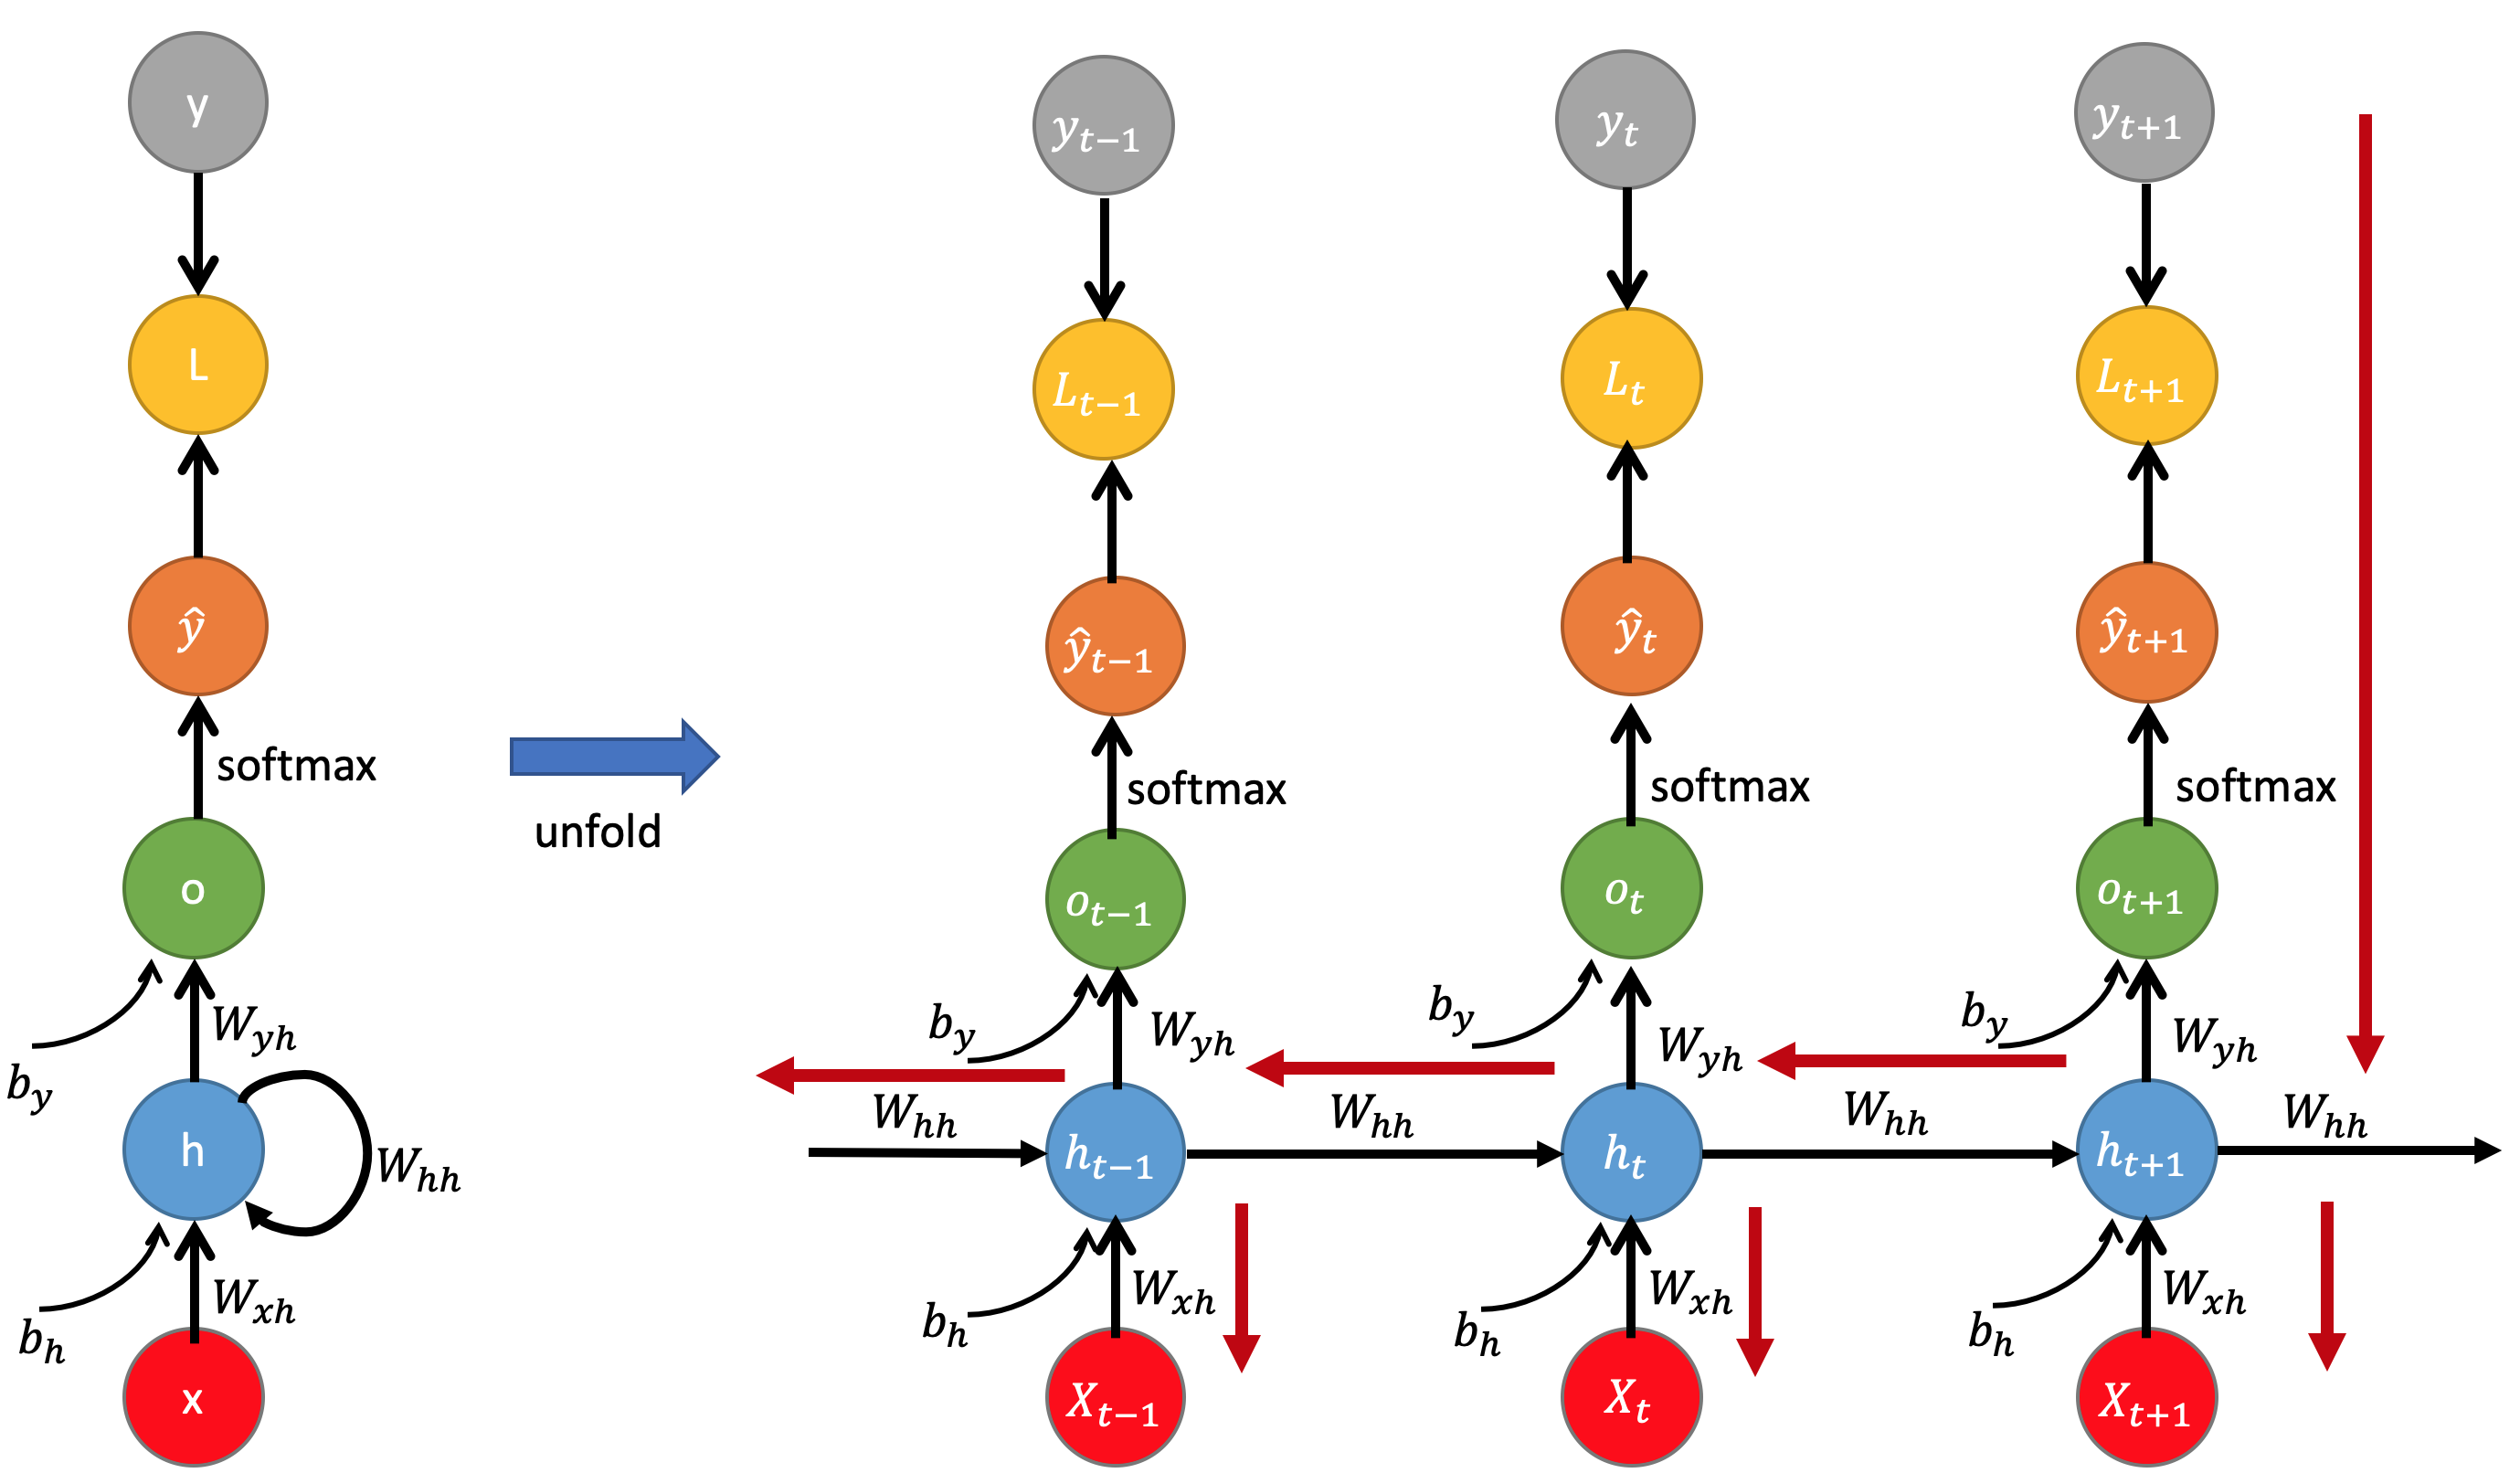
\includegraphics[width=10cm]{Figs/BPTT.png}
\caption{Simple RNN Computational Graph, \href{https://mmuratarat.github.io/2019-02-07/bptt-of-rnn} 
        {source}}

\end{figure}


}

%%%%%%%%%%%%%%%%%%%%%%%%%%%%%%%%%%%%%%%%%%%%%%%%%%%%%%%%%%%%%%%%%%%%%%%%
\frame{\frametitle{Backpropagation Through Time (BPTT)}

\begin{itemize}
    \item
    Suppose that in this example, we have
    $$
    h_t = \mathbin{tanh}(X_t.W_{xh} + h_{t-1}.W_{hh} + b_h)
    $$
    $$
    o_t = h_t.W_{yh} + b_y
    $$
    $$
    y_t = Softmax(o_t)
    $$
    \item
    And our loss function is Log Loss. So as you remember, we have
    $$
    L(y, \Hat{y}) = \sum_{t=1}^{T} L_t(y_t, \Hat{y_t}) = 
    - \sum_{t=1}^{T} y_t \mathbin{log} \Hat{y_t} = 
    - \sum_{t=1}^{T} y_t \mathbin{log} [Softmax(o_t))]
    $$
\end{itemize}
}
%%%%%%%%%%%%%%%%%%%%%%%%%%%%%%%%%%%%%%%%%%%%%%%%%%%%%%%%%%%%%%%%%%%%%%%%######
\frame{\frametitle{Backpropagation Through Time (BPTT)}

\begin{itemize}
    \item
    Now, we are going to calculate derivation of $L$ w.r.t $W_{yh}, W_{hh}, W_{xh}, b_y, b_h$
    \begin{itemize}
        \item Part I: The Straight Ones
        $$
        \frac{\partial L}{\partial W_{yh}} = \sum_{t=1}^{T} \frac{\partial L_t}{\partial W_{yh}}
        $$
        $$ 
        = \sum_{t=1}^{T} \frac{\partial L_t}{\partial \Hat{y_t}} \frac{\partial \Hat{y_t}}{\partial o_t}  \frac{\partial o_t}{\partial W_{yh}}
        $$
        $$
        = \sum_{t=1}^{T} (\Hat{y_t} - y_t) \otimes h_t
        $$
        $$
        \frac{\partial L}{\partial b_{y}} =  \sum_{t=1}^{T} \frac{\partial L_t}{\partial \Hat{y_{t}}} \frac{\partial \Hat{y_{t}}}{\partial o_{t}} \frac{\partial o_{t}}{\partial b_{y}} 
        = \sum_{t=1}^{T} (\Hat{y_t} - y_t)
        $$
    \end{itemize}
    

\end{itemize}
}
%%%%%%%%%%%%%%%%%%%%%%%%%%%%%%%%%%%%%%%%%%%%%%%%%%%%%%%%%%%%%%%%%%%%%%%%
%%%%%%%%%%%%%%%%%%%%%%%%%%%%%%%%%%%%%%%%%%%%%%%%%%%%%%%%%%%%%%%%%%%%%%%%######
\frame{\frametitle{Backpropagation Through Time (BPTT)}

\begin{itemize}
    \item Cont.
    \begin{itemize}
        \item Part II: The Tricky Ones
        $$
        \frac{\partial L_t}{\partial W_{hh}} = \frac{\partial L_t}{\partial \Hat{y_t}} \frac{\partial \Hat{y_t}}{\partial h_t} \frac{\partial h_t}{\partial W_{hh}}
        $$
        we know that $h_{t}$ is a function of $h_{t-1}$ and $W_{hh}$, $h_{t-1}$ itself is a function of $W_{hh}$ and $h_{t-2}$, and so on. Thus, we have
        $$
        \frac{\partial h_t}{\partial W_{hh}} = \left(\frac{\partial h_t}{\partial W_{hh}}\right)_{h_{t-1}} + \frac{\partial h_t}{\partial h_{t-1}} \frac{\partial h_{t-1}}{\partial W_{hh}}
        $$
        $$
        \frac{\partial h_{t-1}}{\partial W_{hh}} = \left(\frac{\partial h_{t-1}}{\partial W_{hh}}\right)_{h_{t-2}} + \frac{\partial h_{t-1}}{\partial h_{t-2}} \frac{\partial h_{t-2}}{\partial W_{hh}}
        $$
        In conclusion, the following equation holds (by substitution)
        $$
        \frac{\partial L_t}{\partial W_{hh}} = \frac{\partial L_t}{\partial \Hat{y_t}} \frac{\partial \Hat{y_t}}{\partial h_t} \left(\sum_{k=1}^t \left(\prod_{j=k}^{t-1}\frac{\partial h_{j+1}}{\partial h_{j}}\right)
        \left(\frac{\partial h_k}{\partial W_{hh}}\right)_{h_{k-1}}\right)
        $$
    \end{itemize}
    

\end{itemize}
}
%%%%%%%%%%%%%%%%%%%%%%%%%%%%%%%%%%%%%%%%%%%%%%%%%%%%%%%%%%%%%%%%%%%%%%%%
\frame{\frametitle{Backpropagation Through Time (BPTT)}

\begin{itemize}
    \item Cont.
        It's also true that
        $$
        \prod_{j=k}^{t-1}\frac{\partial h_{j+1}}{\partial h_{j}} = \frac{\partial h_t}{\partial h_k}
        $$
        That leads us to
        $$
        \frac{\partial L_t}{\partial W_{hh}} = \sum_{k=1}^t \frac{\partial L_t}{\partial \Hat{y_t}} \frac{\partial \Hat{y_t}}{\partial h_t}  
        \frac{\partial h_t}{\partial h_k}
        \left(\frac{\partial h_k}{\partial W_{hh}}\right)_{h_{k-1}}
        $$
        and
        $$
        \frac{\partial L}{\partial W_{hh}} = \sum_{t=1}^{T}\sum_{k=1}^t \frac{\partial L_t}{\partial \Hat{y_t}} \frac{\partial \Hat{y_t}}{\partial h_t}  
        \frac{\partial h_t}{\partial h_k}
        \left(\frac{\partial h_k}{\partial W_{hh}}\right)_{h_{k-1}}
        $$

\end{itemize}
}
%%%%%%%%%%%%%%%%%%%%%%%%%%%%%%%%%%%%%%%%%%%%%%%%%%%%%%%%%%%%%%%%%%%%%%%%
\frame{\frametitle{Backpropagation Through Time (BPTT)}

\begin{itemize}
    \item Cont.
        Similar to the mentioned way, we could compute derivative of $L$ w.r.t $W_{xh}, b_h$ 
        $$
        \frac{\partial L}{\partial W_{xh}} = \sum_{t=1}^{T}\sum_{k=1}^t \frac{\partial L_t}{\partial \Hat{y_t}} \frac{\partial \Hat{y_t}}{\partial h_t}  
        \frac{\partial h_t}{\partial h_k}
        \left(\frac{\partial h_k}{\partial W_{xh}}\right)_{h_{k-1}}
        $$
         $$
        \frac{\partial L}{\partial b_{h}} = \sum_{t=1}^{T}\sum_{k=1}^t \frac{\partial L_t}{\partial \Hat{y_t}} \frac{\partial \Hat{y_t}}{\partial h_t}  
        \frac{\partial h_t}{\partial h_k}
        \left(\frac{\partial h_k}{\partial b_{h}}\right)_{h_{k-1}}
        $$

\end{itemize}
}
%%%%%%%%%%%%%%%%%%%%%%%%%%%%%%%%%%%%%%%%%%%%%%%%%%%%%%%%%%%%%%%%%%%%%%%%
\frame{\frametitle{Backpropagation Through Time (BPTT)}

\begin{figure}[!h]
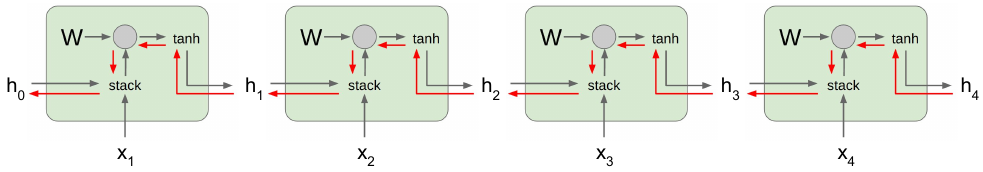
\includegraphics[width=8cm]{Figs/gradient_flow_rnn.png}
\caption{Vanilla RNN Gradient Flow, \href{https://kharshit.github.io/blog/2019/01/04/the-gradient-problem-in-rnn} 
        {source}}

\end{figure}

\begin{itemize}
    \item RNN Training Issues
    \vspace{3mm}
    \begin{itemize}
        \item Computing gradient of $h_0$ involves many factors of $W$ (and repeated 
        $\mathbin{tanh}$)
            \\ What can we do to solve the problem? TBPTT
        \vspace{3mm}
        \item Vanishing $\&$ Exploding gradients
            \\ What can we do to solve exploding? gradient clipping
            \\ What can we do to solve vanishing? changing the structure

    \end{itemize}
    

\end{itemize}
}
%%%%%%%%%%%%%%%%%%%%%%%%%%%%%%%%%%%%%%%%%%%%%%%%%%%%%%%%%%%%%%%%%%%%%%%%
\frame{\frametitle{Truncated Backpropagation Through Time (TBPTT)}
\begin{figure}[!h]
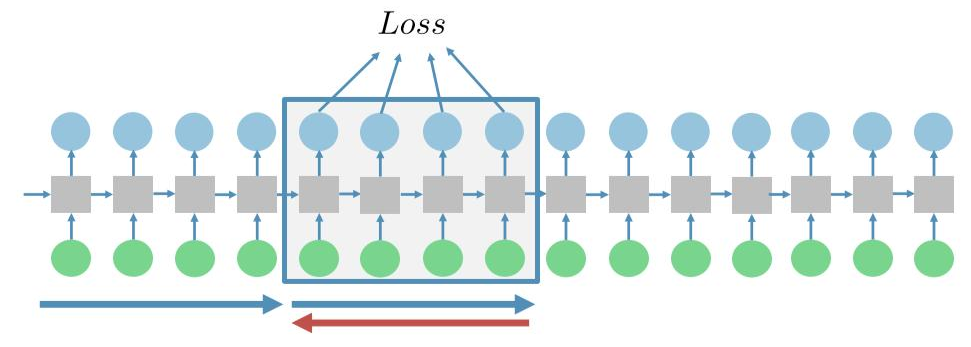
\includegraphics[width=8cm]{Figs/tbptt.png}
\caption{TBPTT for $k_1 = k_2 = 4$, \href{https://www.programmersought.com/article/77613555017/} 
        {source}}

\end{figure}


\begin{itemize}
    \item TBPTT Pseudo Code
    \begin{enumerate}
        \item for $t$ from $1$ to $T$ do
        \item \hspace{1cm}Run the RNN one step
        \item \hspace{1cm}if $t$ divides $k_1$ then
        \item \hspace{1cm}\hspace{1cm}Run BPTT from $t$ down to $t - k_2$
        \item \hspace{1cm}end if
        \item end for 
    \end{enumerate}


\end{itemize}
}
%%%%%%%%%%%%%%%%%%%%%%%%%%%%%%%%%%%%%%%%%%%%%%%%%%%%%%%%%%%%%%%%%%%%%%%%
\frame{\frametitle{RNN Unit}
	
\begin{figure}[!h]
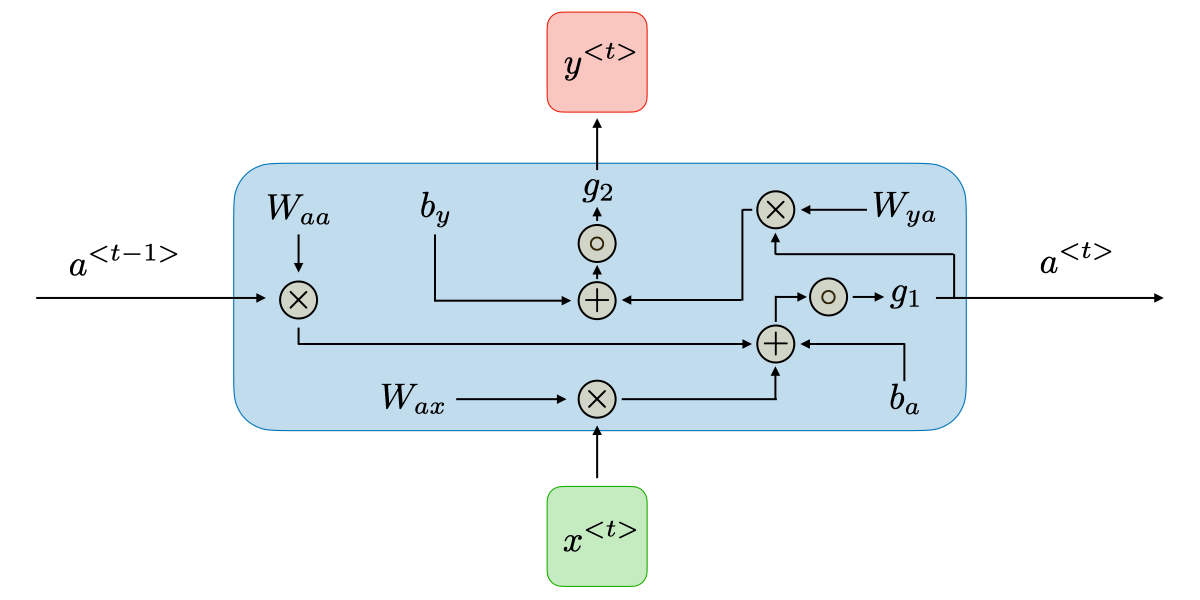
\includegraphics[width=6cm]{Figs/description-block-rnn-ltr.eps}
\caption{RNN Unit, \href{https://stanford.edu/~shervine/teaching/cs-230/cheatsheet-recurrent-neural-networks} 
        {source}}

\end{figure}


\begin{itemize}

	\item 
	For a simple RNN unit we had:

$$
a^{<t>} = g_1(W_{aa}a^{<t-1>} + W_{ax}x^{<t>}+b_a)
\\
\centering y^{<t>} = g_2(W_{ga}a^{<t>}+b_y)
$$

\end{itemize}	


}

%%%%%%%%%%%%%%%%%%%%%%%%%%%%%%%%%%%%%%%%%%%%%%%%%%%%%%%%%%%%%%%%%%%%%%%%%%%%%%%%%%%%%%%%%%%%%%%
%%%%%%%%%%%%%%%%%%%%%%%%%%%%%%%%%%%%%%%%%%%%%%%%%%%%%%%%%%%%%%%%%%%%%%%%######
\frame{\frametitle{Gated Recurrent Unit (GRU)}
	
\begin{figure}[!h]
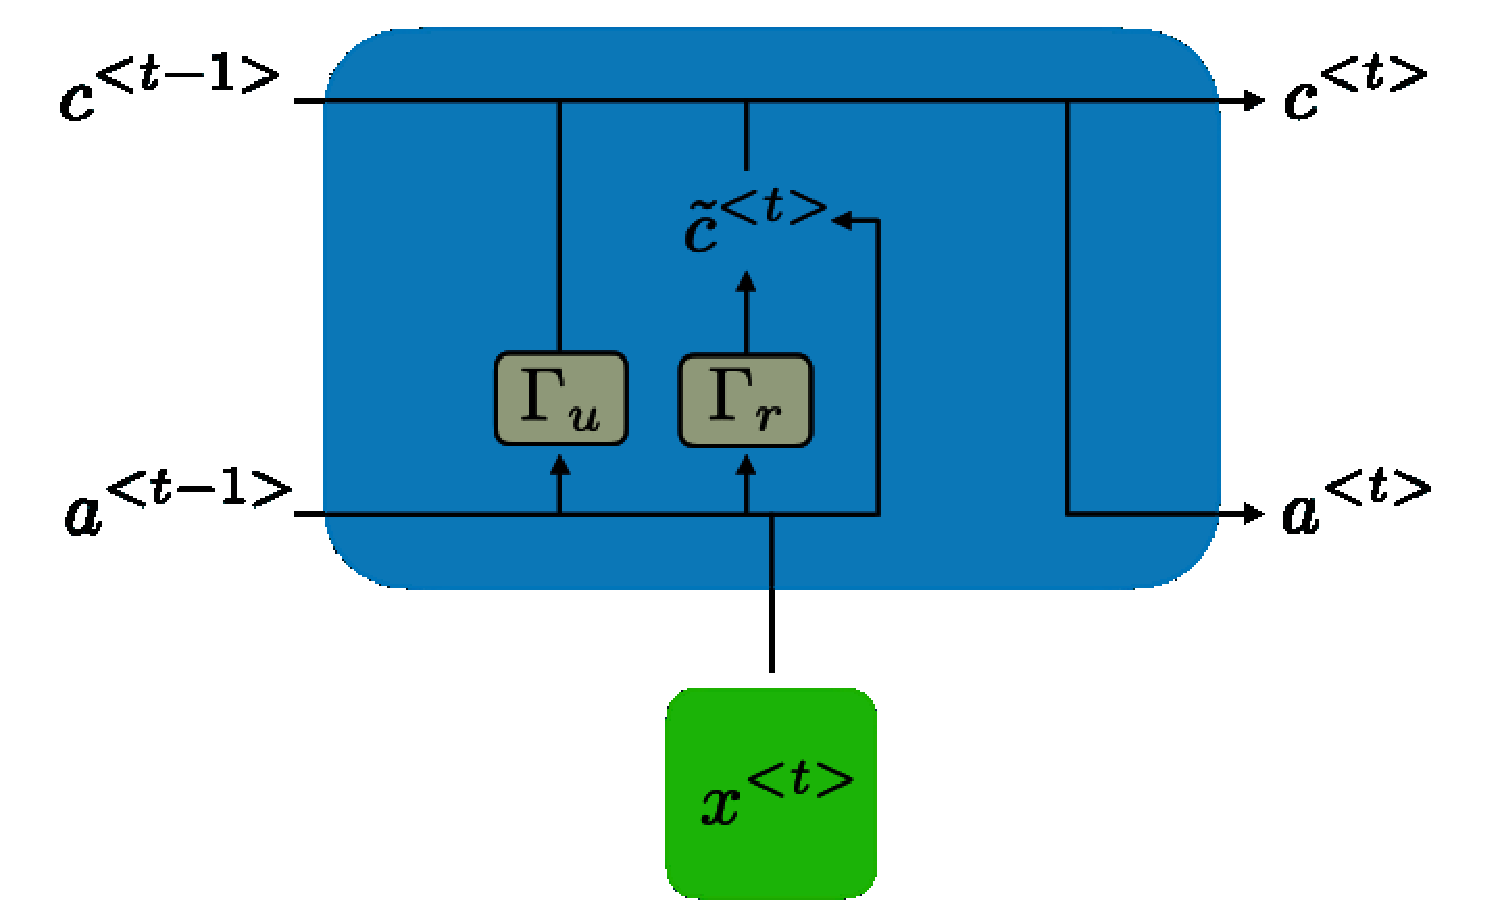
\includegraphics[width=5cm]{Figs/gru-ltr.eps}
\caption{GRU Unit, \href{https://stanford.edu/~shervine/teaching/cs-230/cheatsheet-recurrent-neural-networks} 
        {source}}
\centering
\end{figure}
$$
\Tilde{c}^{<t>} = \tanh(W_{c}[\Gamma_r * a^{<t-1>}, x^{<t>}]+ b_c)
$$
$$
\Gamma_r= \sigma(W_{r}[a^{<t-1>}, x^{<t>}]+b_r)
$$
$$
\Gamma_u= \sigma(W_{u}[a^{<t-1>}, x^{<t>}]+b_u)
$$
$$
c^{<t>} = \Gamma_u * \Tilde{c}^{<t>} + (1-\Gamma_u) * c^{<t-1>}
$$
$$
c^{<t>} = a^{<t>}
$$


}

%%%%%%%%%%%%%%%%%%%%%%%%%%%%%%%%%%%%%%%%%%%%%%%%%%%%%%%%%%%%%%%%%%%%%%%%%%%%%%%%%%%%%%%%%%%%%%%
%%%%%%%%%%%%%%%%%%%%%%%%%%%%%%%%%%%%%%%%%%%%%%%%%%%%%%%%%%%%%%%%%%%%%%%%######
\frame{\frametitle{Long Short-Term Memory (LSTM)}
	
\begin{figure}[!h]
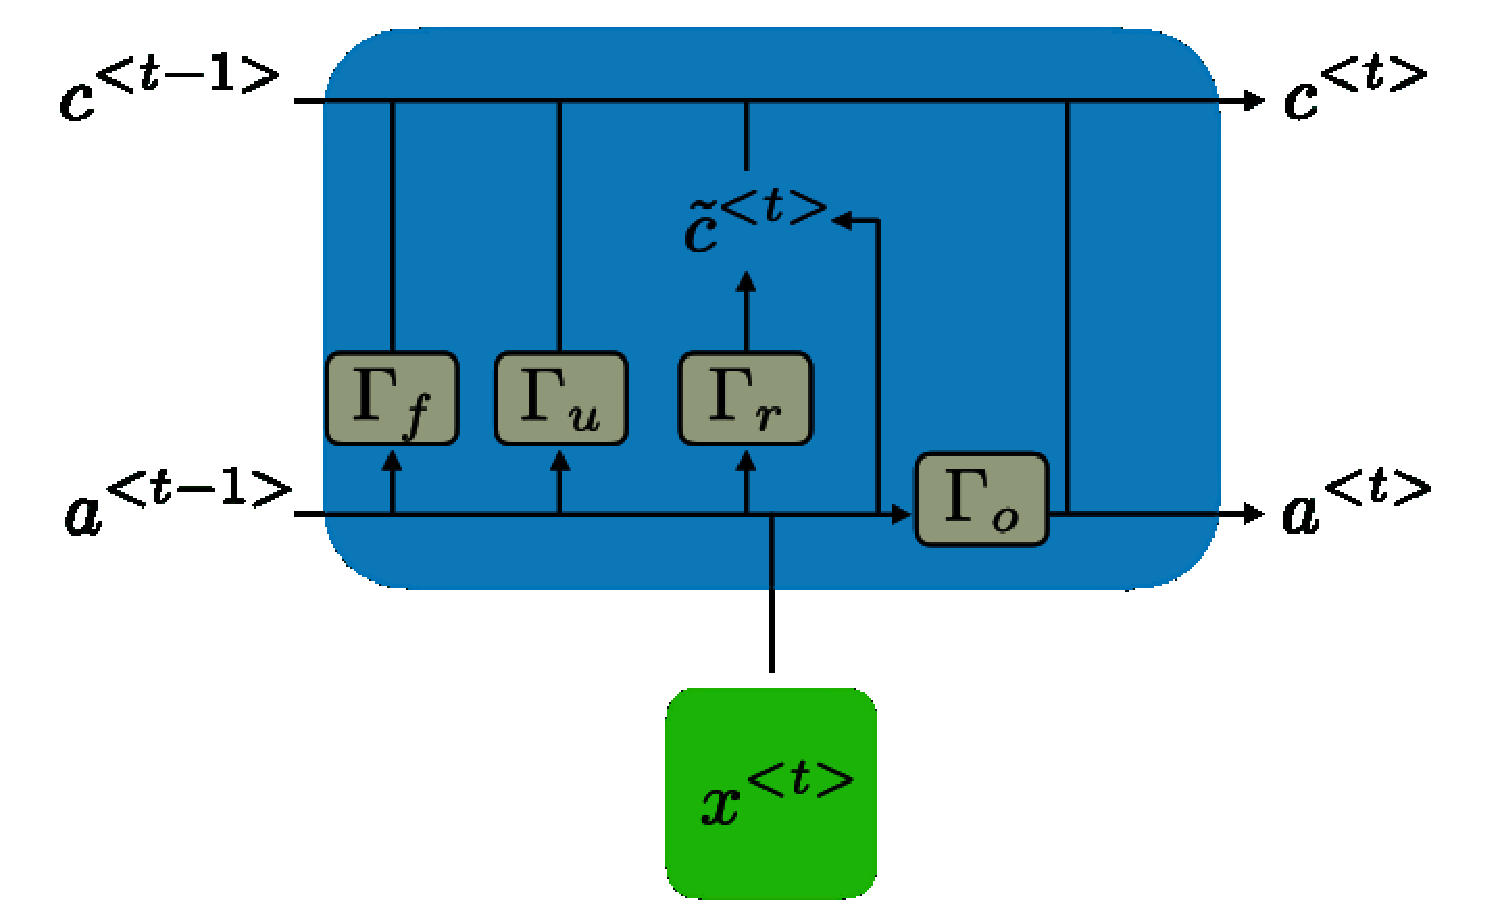
\includegraphics[width=4cm]{Figs/lstm-ltr.eps}
\caption{LSTM Unit, \href{https://stanford.edu/~shervine/teaching/cs-230/cheatsheet-recurrent-neural-networks} 
        {source}}
\end{figure}
$$
\Tilde{c}^{<t>} = \tanh(W_{c}[\Gamma_r * a^{<t-1>}, x^{<t>}]+ b_c)
$$
$$
\Gamma_r= \sigma(W_{r}[a^{<t-1>}, x^{<t>}]+b_r)
$$
$$
\Gamma_u= \sigma(W_{u}[a^{<t-1>}, x^{<t>}]+b_u)
$$
$$
\Gamma_o= \sigma(W_{o}[a^{<t-1>}, x^{<t>}]+b_o)
$$
$$
c^{<t>} = \Gamma_u * \Tilde{c}^{<t>} + (\Gamma_f) * c^{<t-1>}
$$
$$
a^{<t>} = \Gamma_o * c^{<t>}
$$


}

%%%%%%%%%%%%%%%%%%%%%%%%%%%%%%%%%%%%%%%%%%%%%%%%%%%%%%%%%%%%%%%%%%%%%%%%%%%%%%%%%%%%%%%%%%%%%%%
%%%%%%%%%%%%%%%%%%%%%%%%%%%%%%%%%%%%%%%%%%%%%%%%%%%%%%%%%%%%%%%%%%%%%%%%######
\frame{\frametitle{Type of Gates}
	
\begin{itemize}
	\item Update Gate $\Gamma_u$
	\begin{itemize}
		\item How much past should matter
	\end{itemize}

	\item Relevance Gate $\Gamma_r$
 	\begin{itemize}
		\item Drop previous information
	\end{itemize}

	\item Forget gate $\Gamma_f$
 	\begin{itemize}
		\item Erase a cell or not
	\end{itemize}

        \item Output gate $\Gamma_o$
        \begin{itemize}
		\item How much to reveal of a cell
	\end{itemize}

        
\end{itemize}	
	

}

%%%%%%%%%%%%%%%%%%%%%%%%%%%%%%%%%%%%%%%%%%%%%%%%%%%%%%%%%%%%%%%%%%%%%%%%%%%%%%%%%%%%%%%%%%%%%%%
%%%%%%%%%%%%%%%%%%%%%%%%%%%%%%%%%%%%%%%%%%%%%%%%%%%%%%%%%%%%%%%%%%%%%%%%######
\frame{\frametitle{LSTM Walk Through}
\begin{itemize}
    \item The first step in our LSTM is to decide what information we’re going to throw away from the cell state.
\end{itemize}
\begin{figure}[!h]
\centering 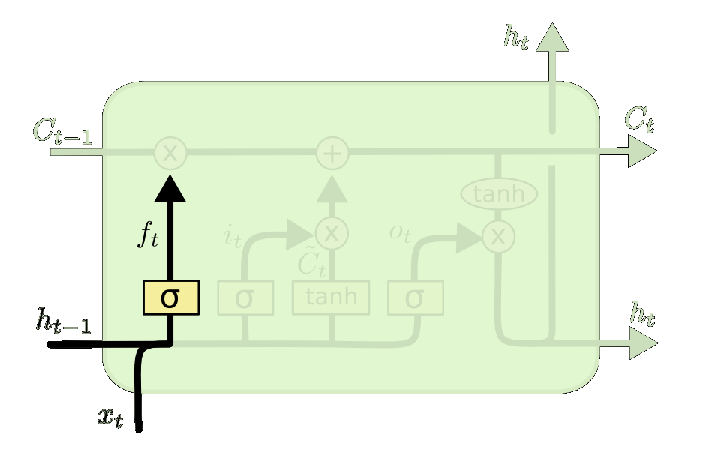
\includegraphics[width=6cm]{Figs/LSTM3-focus-f.eps}
\caption{Forget Gate Layer, \href{https://colah.github.io/posts/2015-08-Understanding-LSTMs/}
        {source}}
\end{figure}
	

}

%%%%%%%%%%%%%%%%%%%%%%%%%%%%%%%%%%%%%%%%%%%%%%%%%%%%%%%%%%%%%%%%%%%%%%%%%%%%%%%%%%%%%%%%%%%%%%%
%%%%%%%%%%%%%%%%%%%%%%%%%%%%%%%%%%%%%%%%%%%%%%%%%%%%%%%%%%%%%%%%%%%%%%%%######
\frame{\frametitle{LSTM Walk Through}
\begin{itemize}
    \item The next step is to decide what new information we’re going to store in the cell state.
\end{itemize}
\begin{figure}[!h]
\centering 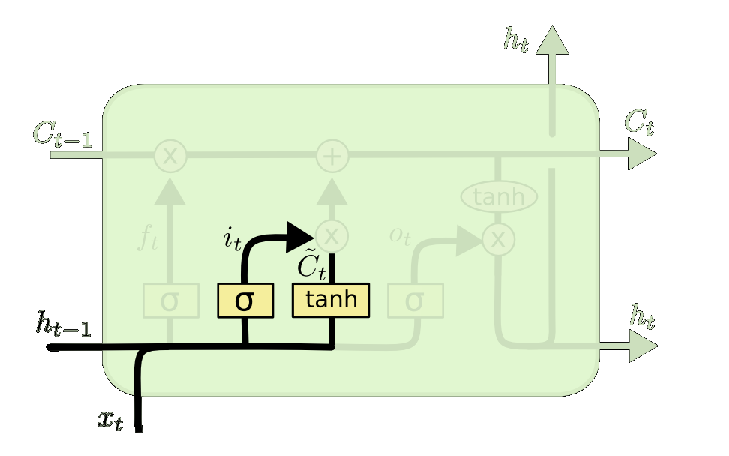
\includegraphics[width=6cm]{Figs/LSTM3-focus-i.eps}
\caption{Input Gate Layer, \href{https://colah.github.io/posts/2015-08-Understanding-LSTMs/}
        {source}}
\end{figure}	

	

}

%%%%%%%%%%%%%%%%%%%%%%%%%%%%%%%%%%%%%%%%%%%%%%%%%%%%%%%%%%%%%%%%%%%%%%%%%%%%%%%%%%%%%%%%%%%%%%%
%%%%%%%%%%%%%%%%%%%%%%%%%%%%%%%%%%%%%%%%%%%%%%%%%%%%%%%%%%%%%%%%%%%%%%%%######
\frame{\frametitle{LSTM Walk Through}
\begin{itemize}
    \item It’s now time to update the old cell state, Ct−1, into the new cell state Ct.
\end{itemize}
\begin{figure}[!h]
\centering 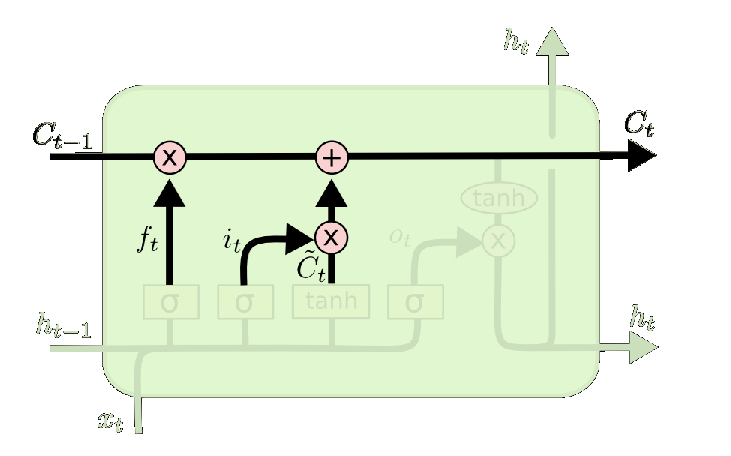
\includegraphics[width=6cm]{Figs/LSTM3-focus-C.eps}
\caption{Update Cell State, \href{https://colah.github.io/posts/2015-08-Understanding-LSTMs/}
        {source}}
\end{figure}	

}

%%%%%%%%%%%%%%%%%%%%%%%%%%%%%%%%%%%%%%%%%%%%%%%%%%%%%%%%%%%%%%%%%%%%%%%%%%%%%%%%%%%%%%%%%%%%%%%
%%%%%%%%%%%%%%%%%%%%%%%%%%%%%%%%%%%%%%%%%%%%%%%%%%%%%%%%%%%%%%%%%%%%%%%%######
\frame{\frametitle{LSTM Walk Through}
\begin{itemize}
    \item Finally, we need to decide what we’re going to output. This output will be based on our cell state
\end{itemize}
\begin{figure}[!h]
\centering 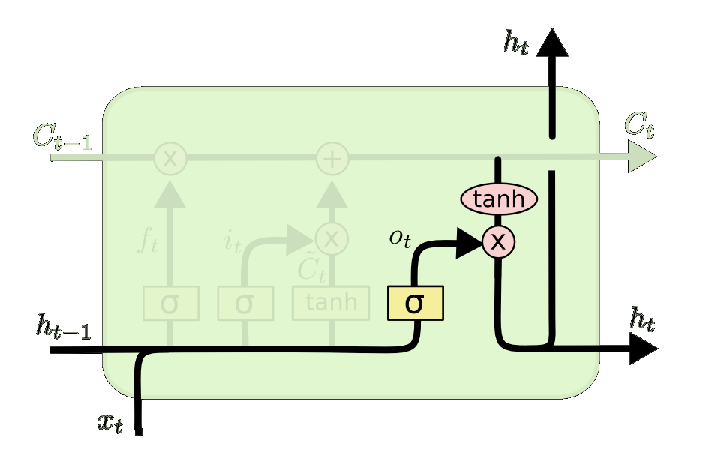
\includegraphics[width=6cm]{Figs/LSTM3-focus-o.eps}
\caption{Output Gate Layer, \href{https://colah.github.io/posts/2015-08-Understanding-LSTMs/}
        {source}}
\end{figure}	

}

%%%%%%%%%%%%%%%%%%%%%%%%%%%%%%%%%%%%%%%%%%%%%%%%%%%%%%%%%%%%%%%%%%%%%%%%%%%%%%%%%%%%%%%%%%%%%%%
%%%%%%%%%%%%%%%%%%%%%%%%%%%%%%%%%%%%%%%%%%%%%%%%%%%%%%%%%%%%%%%%%%%%%%%%######
\frame{\frametitle{Why LSTMs?}
	
\begin{itemize}
	\item The LSTM does have the ability to remove and add information to the cell state.
\vspace{3mm}

	\item The gates in the previous slide let the information to pass through the units.
 
\vspace{3mm}
	\item The gates value are between zero and one and specify how much information should be let through.
\vspace{3mm}
        \item They also somehow solve the vanishing gradient.
        \vspace{3mm}
        
        \item We can use more blocks of them so there will be more information to remember.
        
\end{itemize}	
	

}

%%%%%%%
%%%%%%%%%%%%%%%%%%%%%%%%%%%%%%%%%%%%%%%%%%%%%%%%%%%%%%%%%%%%%%%%%%%%%%%%######
\frame{\frametitle{How LSTMs solve vanishing gradients}
\begin{figure}[!h]
\centering 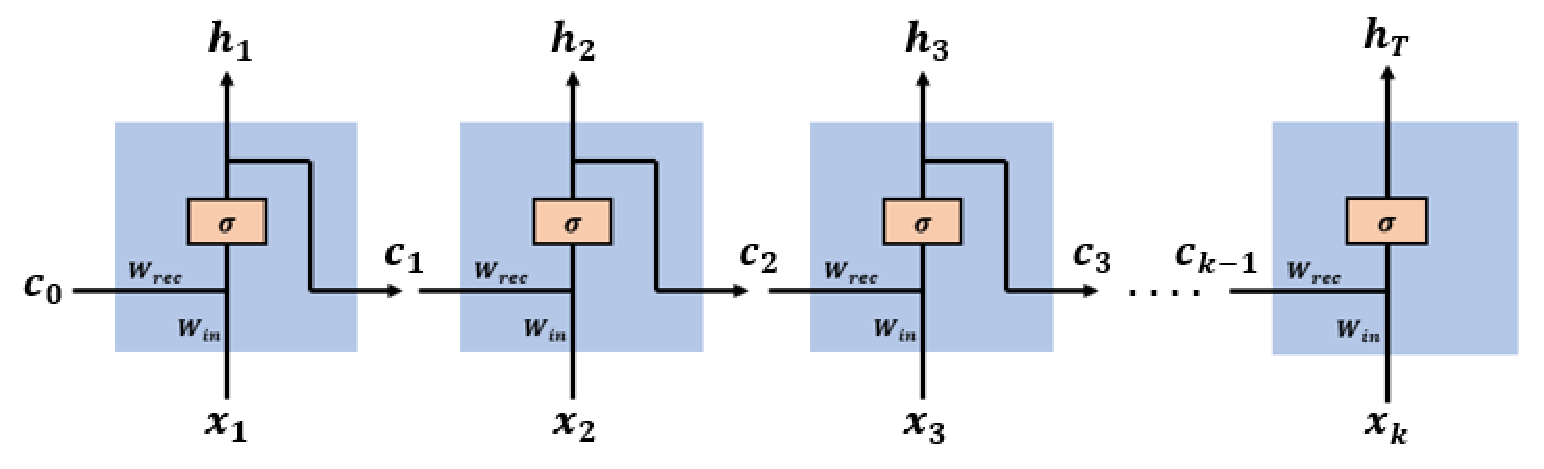
\includegraphics[width=6cm]{Figs/rnn-bp.eps}
\caption{Simple Recurrent Neural Network, \href{https://medium.datadriveninvestor.com/how-do-lstm-networks-solve-the-problem-of-vanishing-gradients-a6784971a577}
        {source}}
\end{figure}
$$
\frac{\partial L}{\partial W} = \sum_{t=1}^{T} \frac{\partial L_t}{\partial W}
$$
\begin{align*}\label{eq:pareto mle2}
\frac{\partial L_k}{\partial W} = \frac{\partial L_k}{\partial h_k} \frac{\partial h_k}{\partial c_k} \dots \frac{\partial c_2}{\partial c_1} \frac{\partial c_1}{\partial W} 
 = \frac{\partial L_k}{\partial h_k} \frac{\partial h_k}{\partial c_k} (\prod_{t=2}^{k} \frac{\partial c_t}{\partial c_{t-1}}) \frac{\partial c_1}{\partial W}
\end{align*}

$$
\frac{\partial c_t}{\partial c_{t-1}} = \sigma'(W_{rec}.c_{t-1} + W_{in}.x_t)W_{rec}
$$
	

}

%%%%%%%%%%%%%%%%%%%%%%%%%%%%%%%%%%%%%%%%%%%%%%%%%%%%%%%%%%%%%%%%%%%%%%%%%%%%%%%%%%%%%%%%%%%%%%%
%%%%%%%%%%%%%%%%%%%%%%%%%%%%%%%%%%%%%%%%%%%%%%%%%%%%%%%%%%%%%%%%%%%%%%%%######
\frame{\frametitle{How LSTMs solve vanishing gradients}
\begin{align*}\label{eq:pareto mle2}
\frac{\partial L_k}{\partial W} = \frac{\partial L_k}{\partial h_k} \frac{\partial h_k}{\partial c_k} (\prod_{t=2}^{k} \sigma'(W_{rec}.c_{t-1} + W_{in}.x_t)W_{rec}) \frac{\partial c_1}{\partial W}
\end{align*}

\begin{itemize}
\item For lagre K the gradient tends to vanish or if $W_{rec}$ is large enough it cause exploding gradient which is solved by \textit{Gradient Clipping}.
\end{itemize}

	

}

%%%%%%%%%%%%%%%%%%%%%%%%%%%%%%%%%%%%%%%%%%%%%%%%%%%%%%%%%%%%%%%%%%%%%%%%%%%%%%%%%%%%%%%%%%%%%%%
%%%%%%%%%%%%%%%%%%%%%%%%%%%%%%%%%%%%%%%%%%%%%%%%%%%%%%%%%%%%%%%%%%%%%%%%######
\frame{\frametitle{How LSTMs solve vanishing gradients}
\begin{itemize}
\item In LSTM we also have

\begin{align*}\label{eq:pareto mle2}
\frac{\partial L_k}{\partial W} =  \frac{\partial L_k}{\partial h_k} \frac{\partial h_k}{\partial c_k} (\prod_{t=2}^{k} \frac{\partial c_t}{\partial c_{t-1}}) \frac{\partial c_1}{\partial W}
\end{align*}
\item But 
$$
c^{t} = \Gamma_u * \Tilde{c}^{t} + (\Gamma_f) * c^{t-1}
$$
$$
\frac{\partial c_t}{\partial c_{t-1}} = \frac{\partial \Gamma_f}{\partial c_{t-1}}.c_{t-1} + \Gamma_f + \frac{\partial \Gamma_u}{\partial c_{t-1}}.\Tilde{c_{t}} + \frac{\partial \Tilde{c_t}}{\partial c_{t-1}}.\Gamma_u
$$

\item Consider that the \textit{forget gate} is added to other terms and allows better control of gradient values. But it doesn't guarantee that there is no vanishing or exploding in gradient.
\end{itemize}



}

%%%%%%%%%%%%%%%%%%%%%%%%%%%%%%%%%%%%%%%%%%%%%%%%%%%%%%%%%%%%%%%%%%%%%%%%%%%%%%%%%%%%%%%%%%%%%%%
%%%%%%%%%%%%%%%%%%%%%%%%%%%%%%%%%%%%%%%%%%%%%%%%%%%%%%%%%%%%%%%%%%%%%%%%######
\frame{\frametitle{Bidirectional RNN}
\begin{itemize}
\item How to get information from future?
\end{itemize}
\begin{figure}[!h]
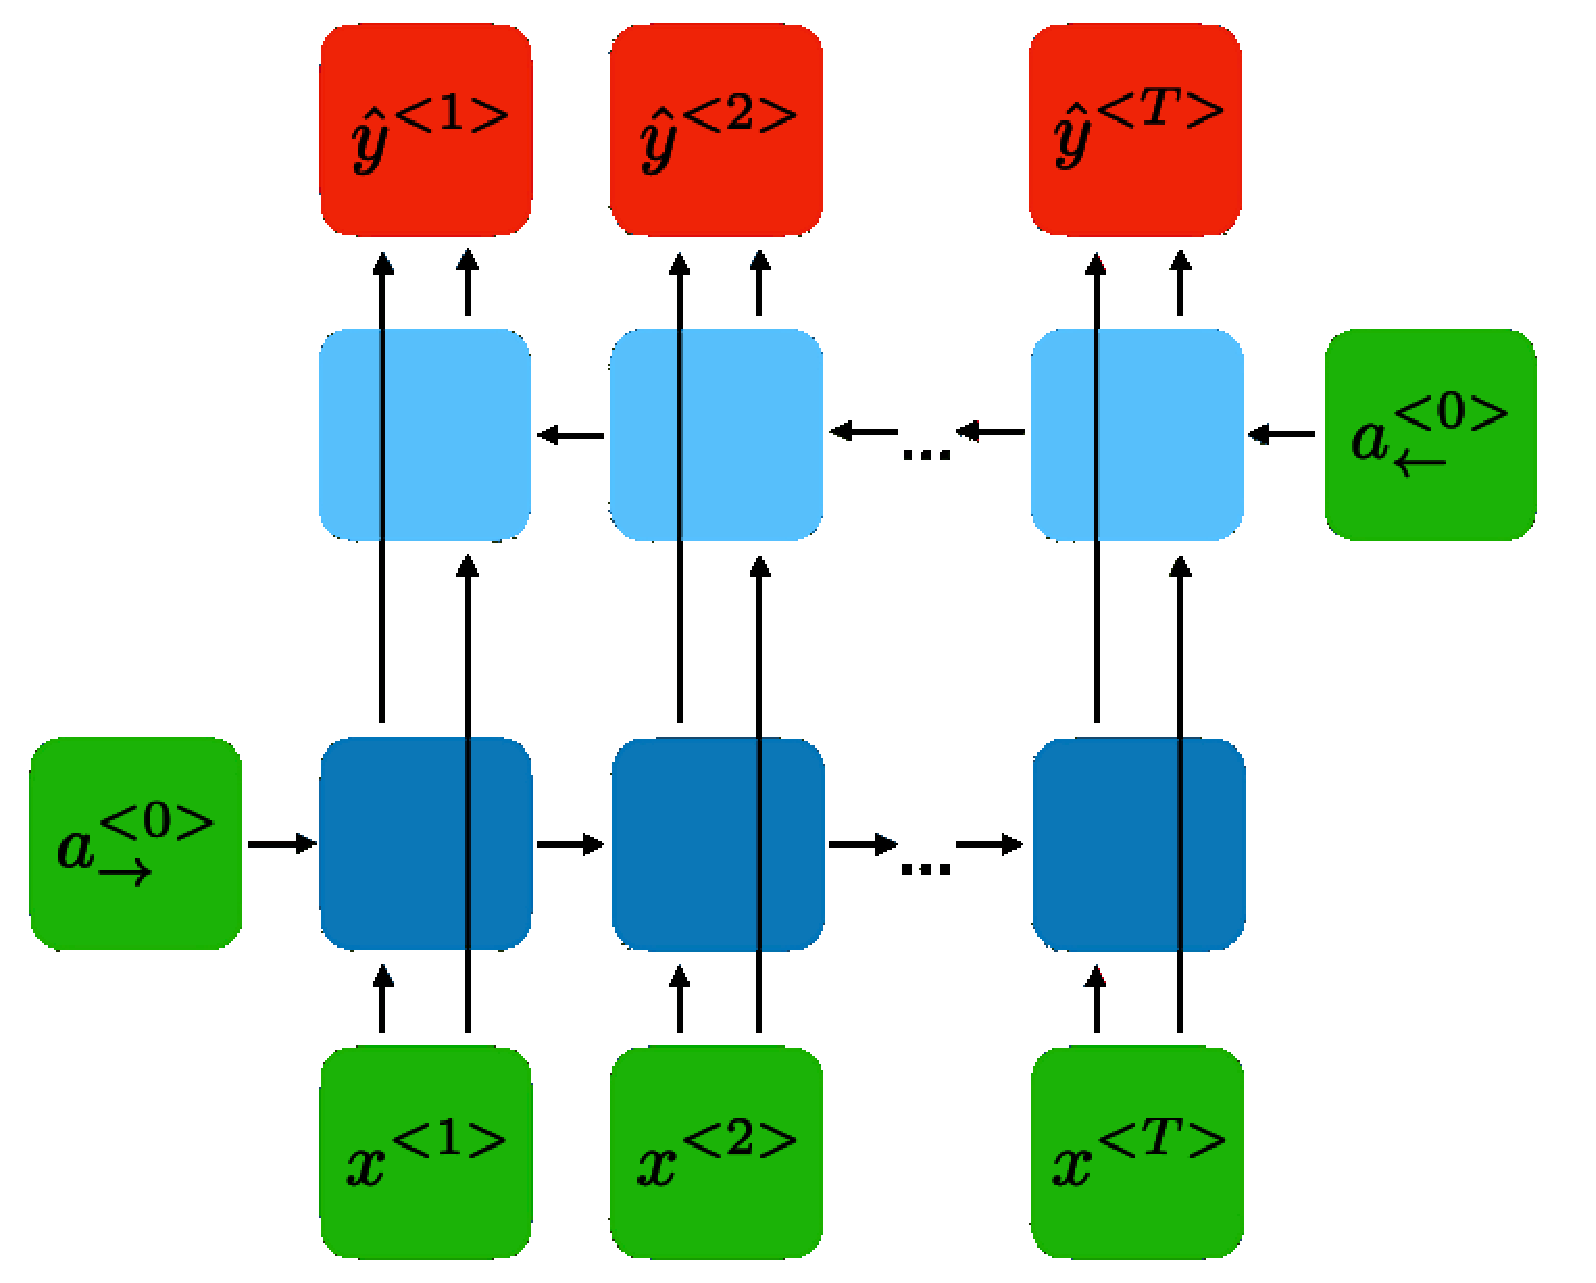
\includegraphics[width=5cm]{Figs/bidirectional-rnn-ltr.eps}
\caption{BRNN, \href{https://stanford.edu/~shervine/teaching/cs-230/cheatsheet-recurrent-neural-networks} 
        {source}}
\centering
\end{figure}

$$
y^{<t>} = g(W_y[\vec{a}^{<t>},\: \cev{a}^{<T-t>}] + b_y)
$$


}

%%%%%%%%%%%%%%%%%%%%%%%%%%%%%%%%%%%%%%%%%%%%%%%%%%%%%%%%%%%%%%%%%%%%%%%%%%%%%%%%%%%%%%%%%%%%%%%
%%%%%%%%%%%%%%%%%%%%%%%%%%%%%%%%%%%%%%%%%%%%%%%%%%%%%%%%%%%%%%%%%%%%%%%%######
\frame{\frametitle{Bidirectional RNN}

\begin{itemize}
    \item They are usually used in natural language processing.

\vspace{3mm}
    
    \item They are powerful for modeling dependencies between words and phrases in both directions of the sequence because every component of an input sequence has information from both the past and present.


\end{itemize}


}

%%%%%%%%%%%%%%%%%%%%%%%%%%%%%%%%%%%%%%%%%%%%%%%%%%%%%%%%%%%%%%%%%%%%%%%%%%%%%%%%%%%%%%%%%%%%%%%
%%%%%%%%%%%%%%%%%%%%%%%%%%%%%%%%%%%%%%%%%%%%%%%%%%%%%%%%%%%%%%%%%%%%%%%%######
\frame{\frametitle{Back-propagation in BRNN}
\begin{itemize}
\item It is exactly the same as simple RNN
\end{itemize}
\begin{figure}[!h]
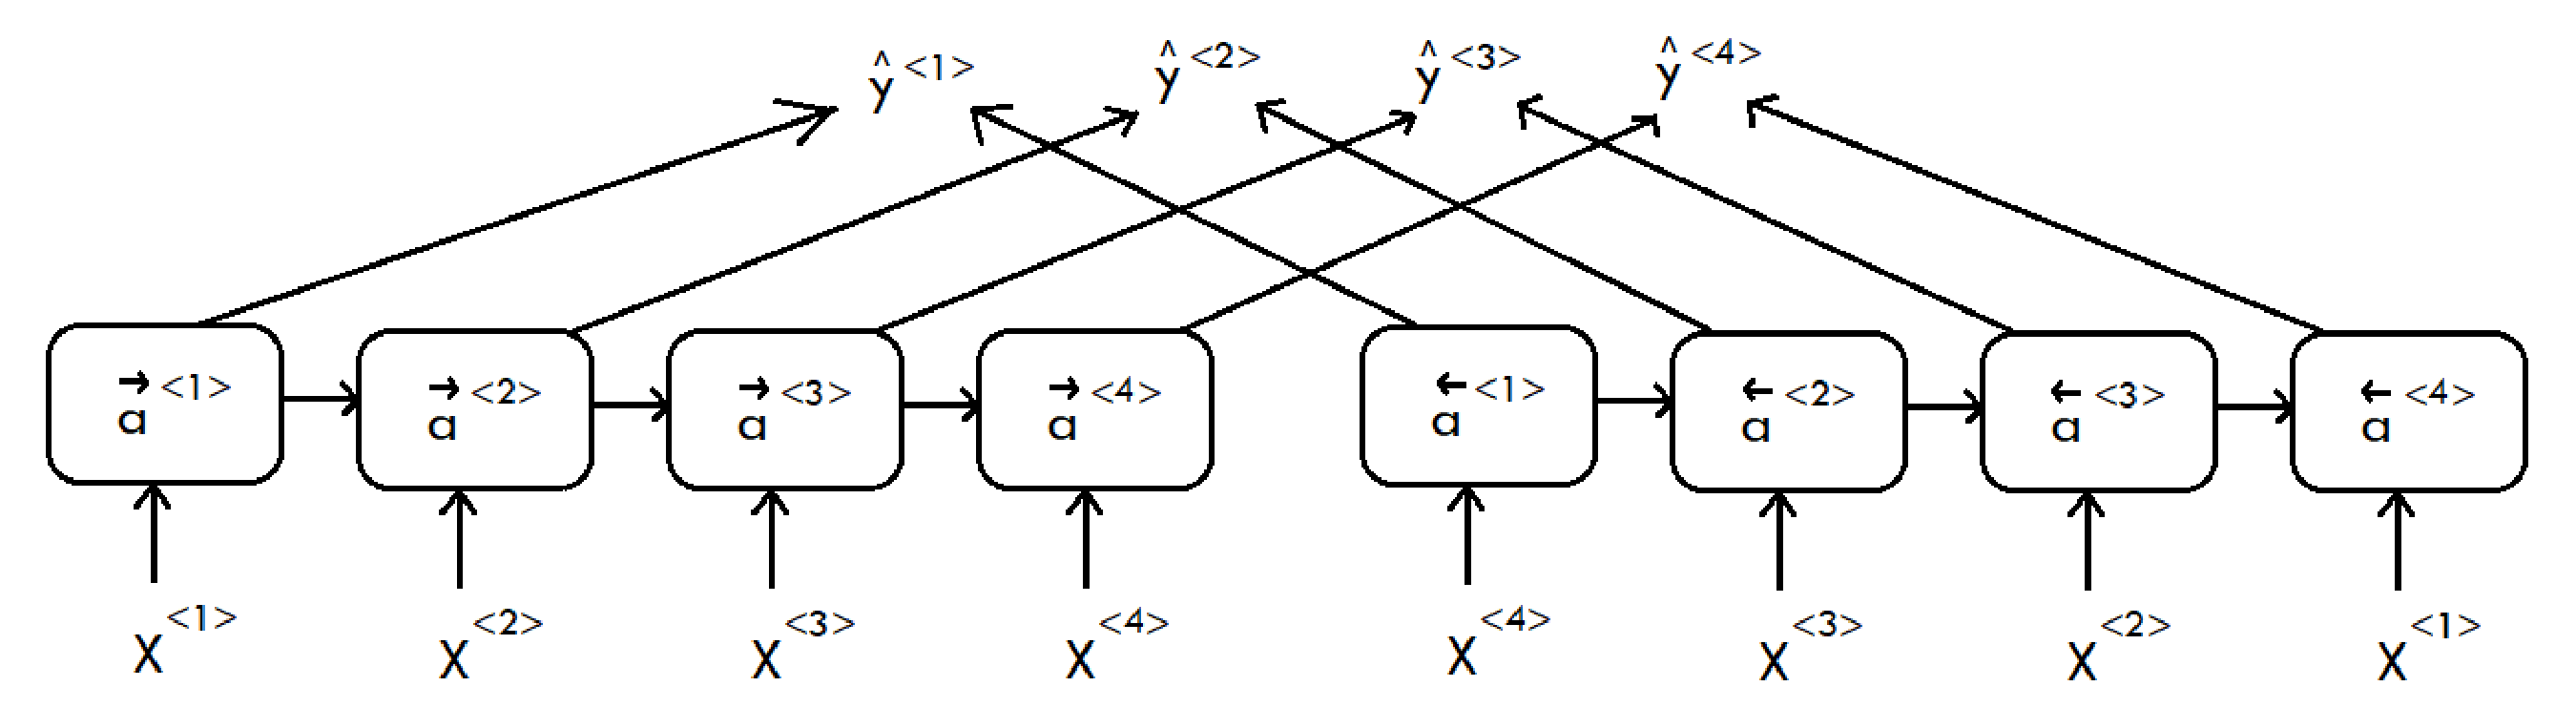
\includegraphics[width=8cm]{Figs/bpbbrn.eps}
\caption{BRNN, \href{https://ai.stackexchange.com/questions/24013/how-does-back-propagation-through-time-work-for-optimizing-the-weights-of-a-bidi} 
        {source}}
\centering
\end{figure}

}
%%%%%%%%%%%%%%%%%%%%%%%%%%%%%%%%%%%%%%%%%%%%%%%%%%%%%%%%%%%%%%%%%%%%%%%%%%%%%%%%%%%%%%%%%%
\frame{\frametitle{Encoder-Decoder}

\begin{itemize}
\item If we want an output of variable length with respect to the
input(e.g. Machine Translation), what should we do?
\vspace{3mm}
\item Can we use RNN for tasks where we have a sequence as input and
we want another sequence as output? Alignment problem.
\end{itemize}
\begin{center}
    Encoder-Decoder architecture could be a solution.
\end{center}

\begin{figure}[!h]
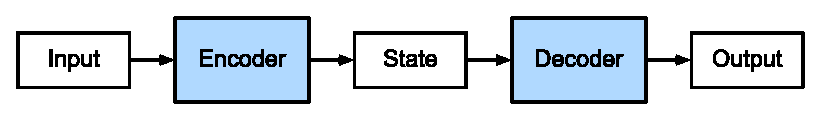
\includegraphics[width=7cm]{Figs/encoder-decoder.eps}
\caption{Encoder-Decoder Architecture, \href{https://d2l.ai/chapter\_recurrent-modern/encoder-decoder.html} 
        {source}}
\end{figure}

}
%%%%%%%%%%%%%%%%%%%%%%%%%%%%%%%%%%%%%%%%%%%%%%%%%%%%%%%%%%%%%%%%%%%%%%%%%%%%%%%%%%%%%
\frame{\frametitle{Encoder-Decoder}

\begin{figure}[!h]
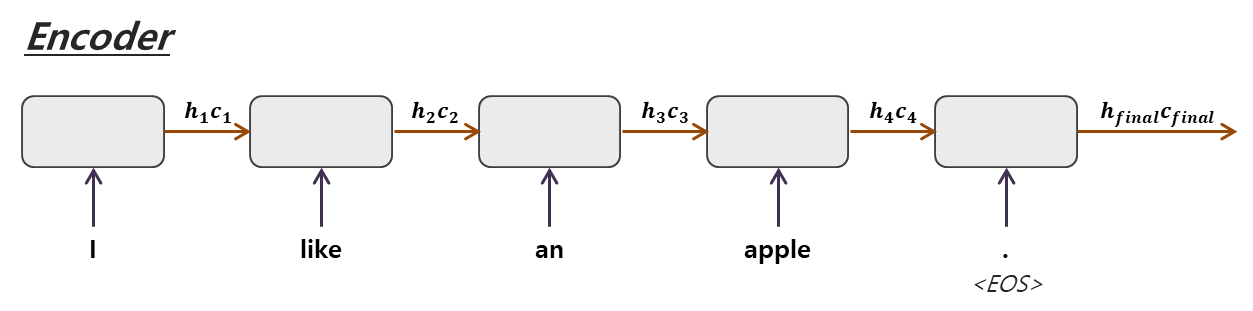
\includegraphics[width=8cm]{Figs/encoder.png}
\caption{Encoder, \href{https://yjjo.tistory.com/35} 
        {source}}
\end{figure}

\begin{itemize}
        \item \textbf{Encoder:} Encoder processes the input sequence and compresses the information into a fixed length vector, known as the context vector. 
\end{itemize}

}
%%%%%%%%%%%%%%%%%%%%%%%%%%%%%%%%%%%%%%%%%%%%%%%%%%%%%%%%%%%%%%%%%%%%%%%%%%%%%%%%%%%%%
\frame{\frametitle{Encoder-Decoder}

\begin{figure}[!h]
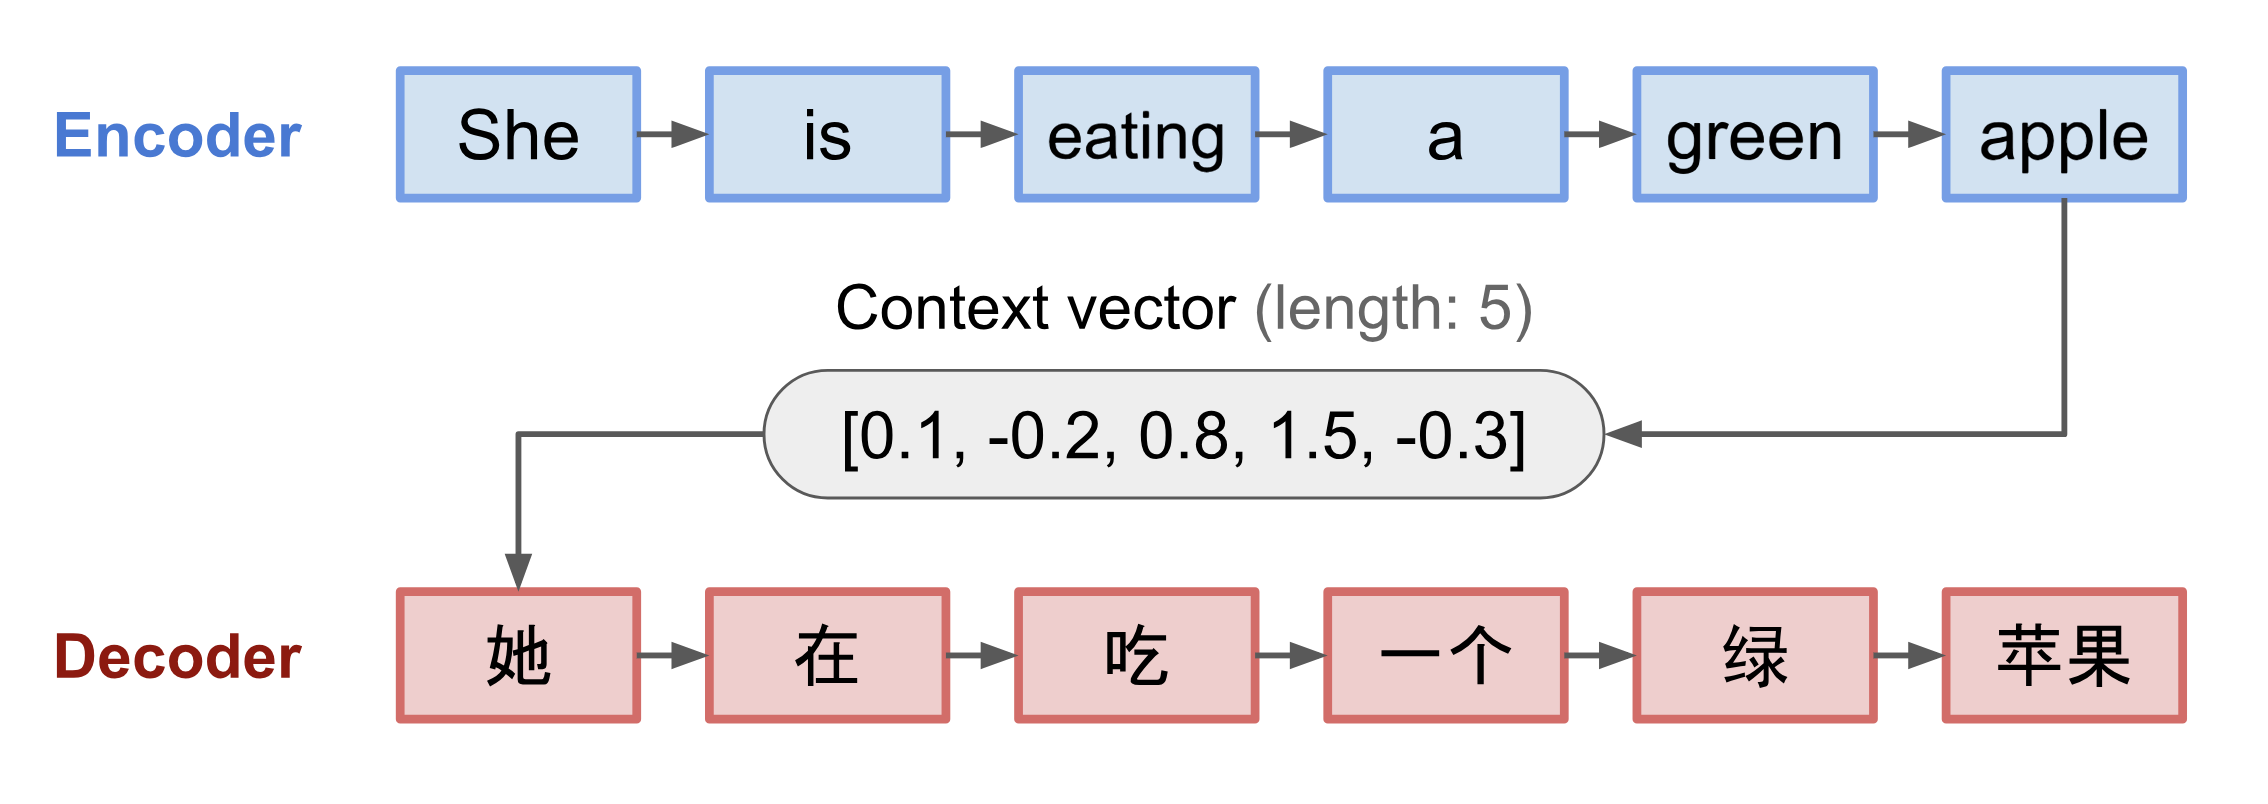
\includegraphics[width=8cm]{Figs/encoder-decoder-example.png}
\caption{Context Vector, \href{https://lilianweng.github.io/posts/2018-06-24-attention/} 
        {source}}
\end{figure}

\begin{itemize}
        \item \textbf{Context Vector:} This representation is expected to be a good summary of the meaning of the whole source sequence. (The early work only used the last state of the encoder network as the context vector.)
\end{itemize}

}
%%%%%%%%%%%%%%%%%%%%%%%%%%%%%%%%%%%%%%%%%%%%%%%%%%%%%%%%%%%%%%%%%%%%%%%%%%%%%%%%%%%%%
\frame{\frametitle{Encoder-Decoder}

\begin{figure}[!h]
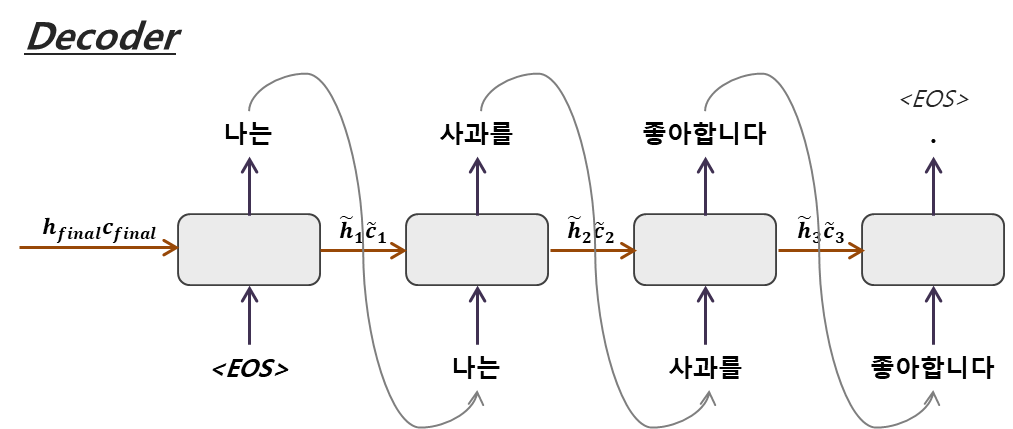
\includegraphics[width=8cm]{Figs/decoder.png}
\caption{Decoder, \href{https://yjjo.tistory.com/35} 
        {source}}
\end{figure}

\begin{itemize}
        \item \textbf{Decoder:} Decoder is initialized with the context vector to output the desired target sequence.
\end{itemize}
}
%%%%%%%%%%%%%%%%%%%%%%%%%%%%%%%%%%%%%%%%%%%%%%%%%%%%%%%%%%%%%%%%%%%%%%%%%%%%%%%%%%%%%
\frame{\frametitle{Encoder-Decoder Limitations}

\begin{itemize}
        \item Slow convergence in training. How to solve it? Teacher Forcing.
\end{itemize}

\begin{figure}[!h]
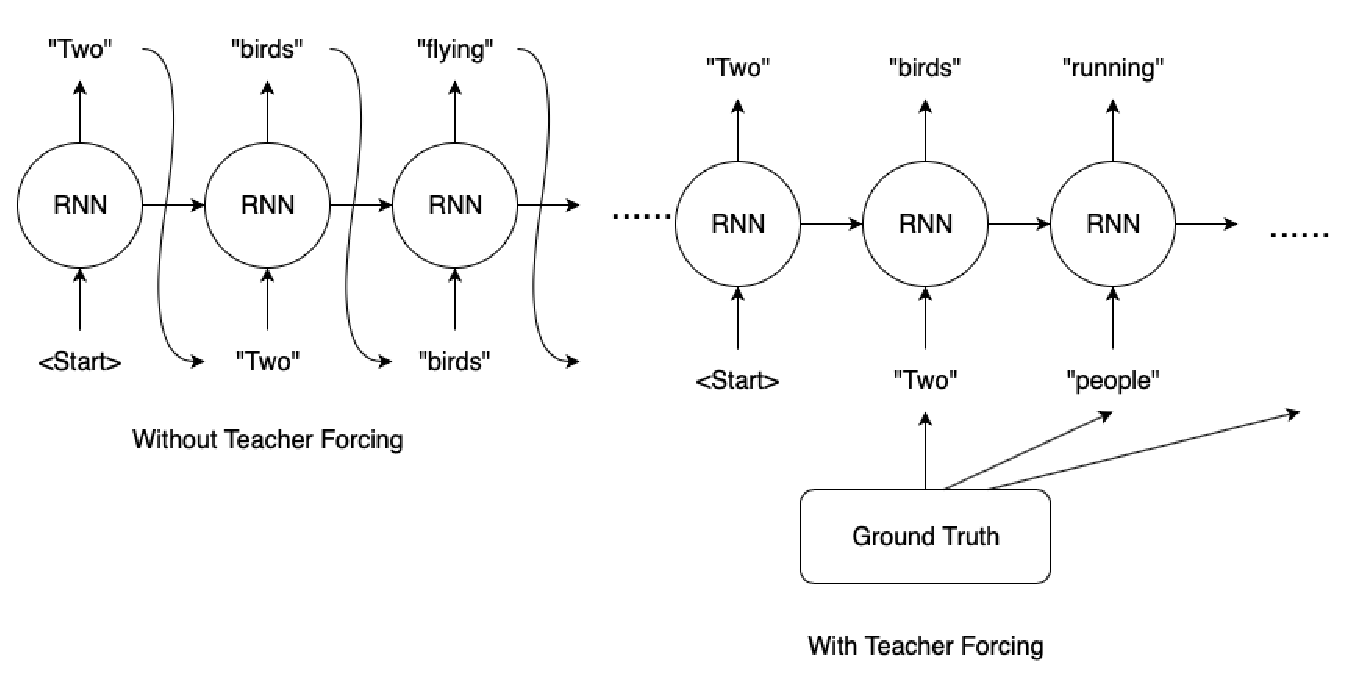
\includegraphics[width=10cm]{Figs/tf_ende.eps}
        \caption{Teacher Forcing In Decoder Side, \href{https://towardsdatascience.com/what-is-teacher-forcing-3da6217fed1c} 
        {source}}
\end{figure}

}
%%%%%
%%%%%%%%%%%%%%%%%%%%%%%%%%%%%%%%%%%%%%%%%%%%%%%%%%%%%%%%%%%%%%%%%%%%%%%%######
\frame{\frametitle{Teacher Forcing}

\begin{itemize}

\item Teacher forcing is a method for training recurrent neural networks more efficiently.
\vspace{3mm}
\item Teacher forcing works by using the actual output at the current time step $y^{(t-1)}$ as input in the next time step, rather than the $o^{(t-1)}$generated by the network.

\end{itemize}
\begin{figure}[!h]
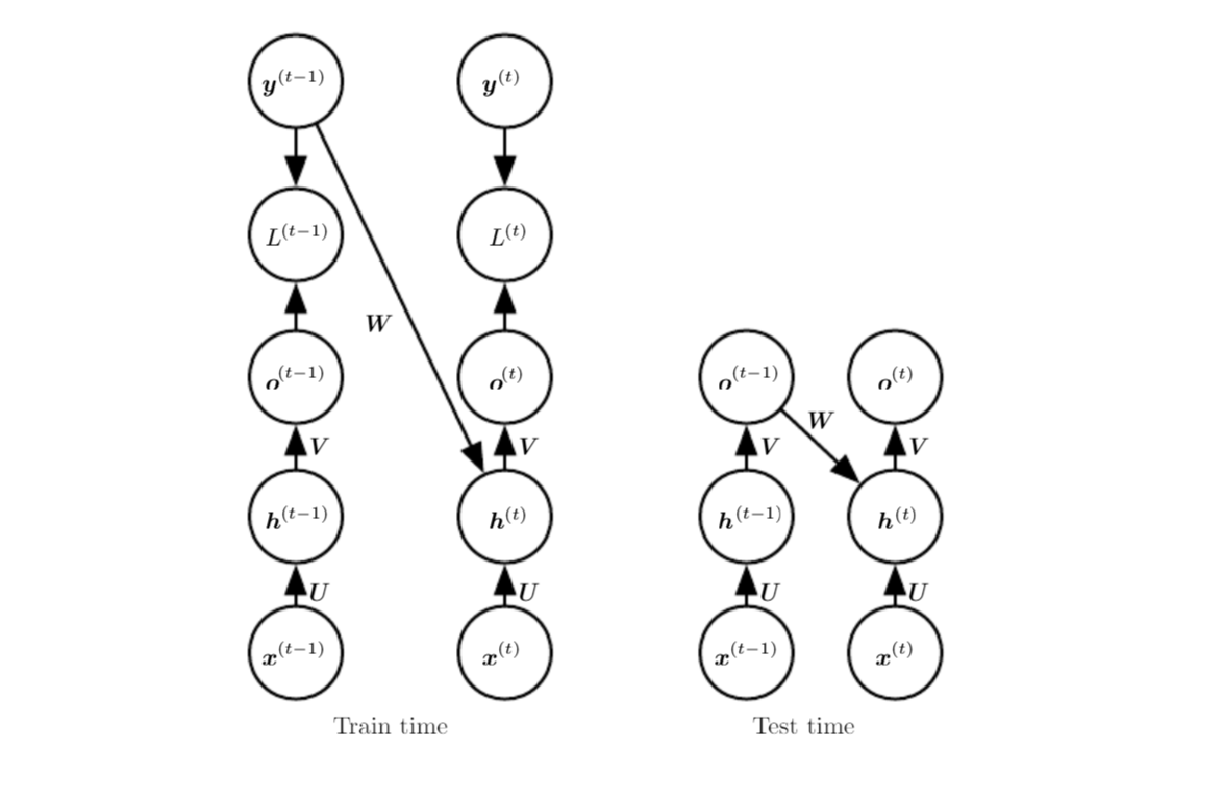
\includegraphics[width=8cm]{Figs/fig10-6.eps}
\caption{Teacher Forcing, \href{https://www.arashash.com/2020-02-23-deeplearning-ch10-lect2/} 
        {source}}
\centering
\end{figure}

}
%%%%%%%%%%%%%%%%%%%%%%%%%%%%%%%%%%%%%%%%%%%%%%%%%%%%%%%%%%%%%%%%%%%%%%%%%%%%%%%%%%%%%%%%%%%%%%%
%%%%%%%%%%%%%%%%%%%%%%%%%%%%%%%%%%%%%%%%%%%%%%%%%%%%%%%%%%%%%%%%%%%%%%%%######
\frame{\frametitle{Teacher Forcing}

\begin{itemize}

\item The problem with RNNs is that we need previous time step output as input for next time step.
\vspace{5mm}
\item This technique allows us to prevent backpropagation through time which was complex and time-consuming.
\vspace{5mm}
\item With teacher forcing the model will be trained faster.
\vspace{5mm}
\item During inference, since there is usually no ground truth available, the RNN model will need to feed its own previous prediction back to itself for the next prediction.
\vspace{5mm}
\end{itemize}

}
%%%%%%%%%%%%%%%%%%%%%%%%%%%%%%%%%%%%%%%%%%%%%%%%%%%%%%%%%%%%%%%%%%%%%%%%%%%%%%%%%%%%%
%%%%%%%%%%%%%%%%%%%%%%%%%%%%%%%%%%%%%%%%%%%%%%%%%%%%%%%%%%%%%%%%%%%%%%%%%%%%%%%%%%%%%
\frame{\frametitle{Encoder-Decoder Limitations}
\begin{figure}[!h]
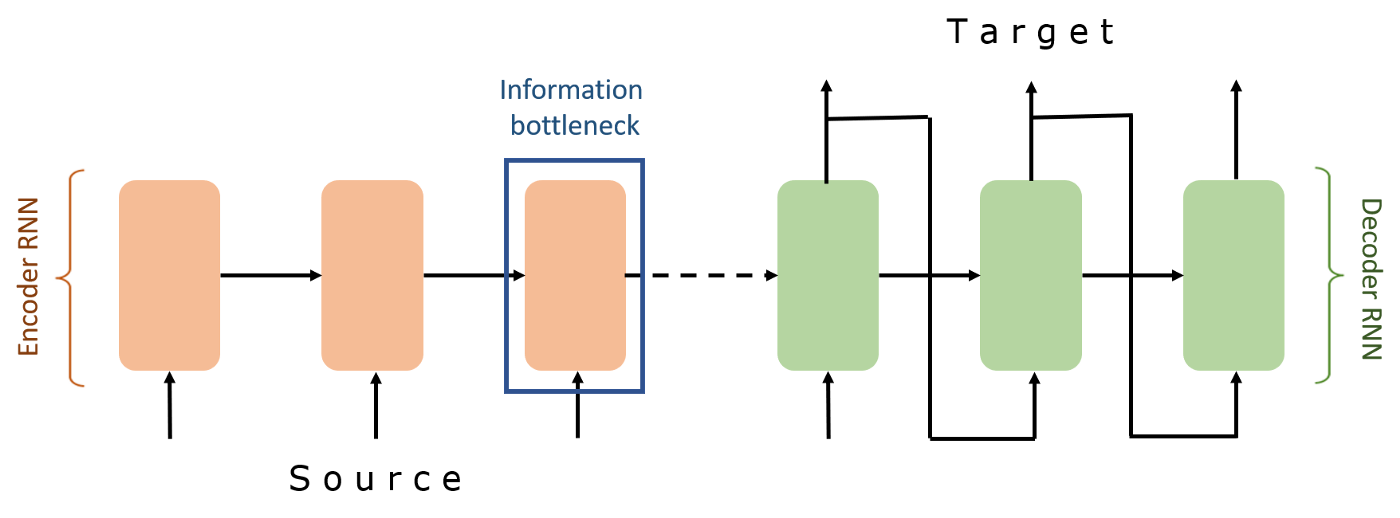
\includegraphics[width=8cm]{Figs/bottleneck.png}
        \caption{Bottleneck Phenomenon, \href{https://towardsdatascience.com/attention-and-its-different-forms-7fc3674d14dc} 
        {source}}
\end{figure}

\begin{itemize}
        \item The context vector is bottleneck. 
        By increasing the length of the input sequence, the model captures the essential information roughly. How to solve it? Attention! Define and use the the context vector better.
\end{itemize}

}
%%%%%%%%%%%%%%%%%%%%%%%%%%%%%%%%%%%%%%%%%%%%%%%%%%%%%%%%%%%%%%%%%%%%%%%%%%%%%%%%%%%%%
\frame{\frametitle{Review: Machine Translation}
\begin{figure}[!h]
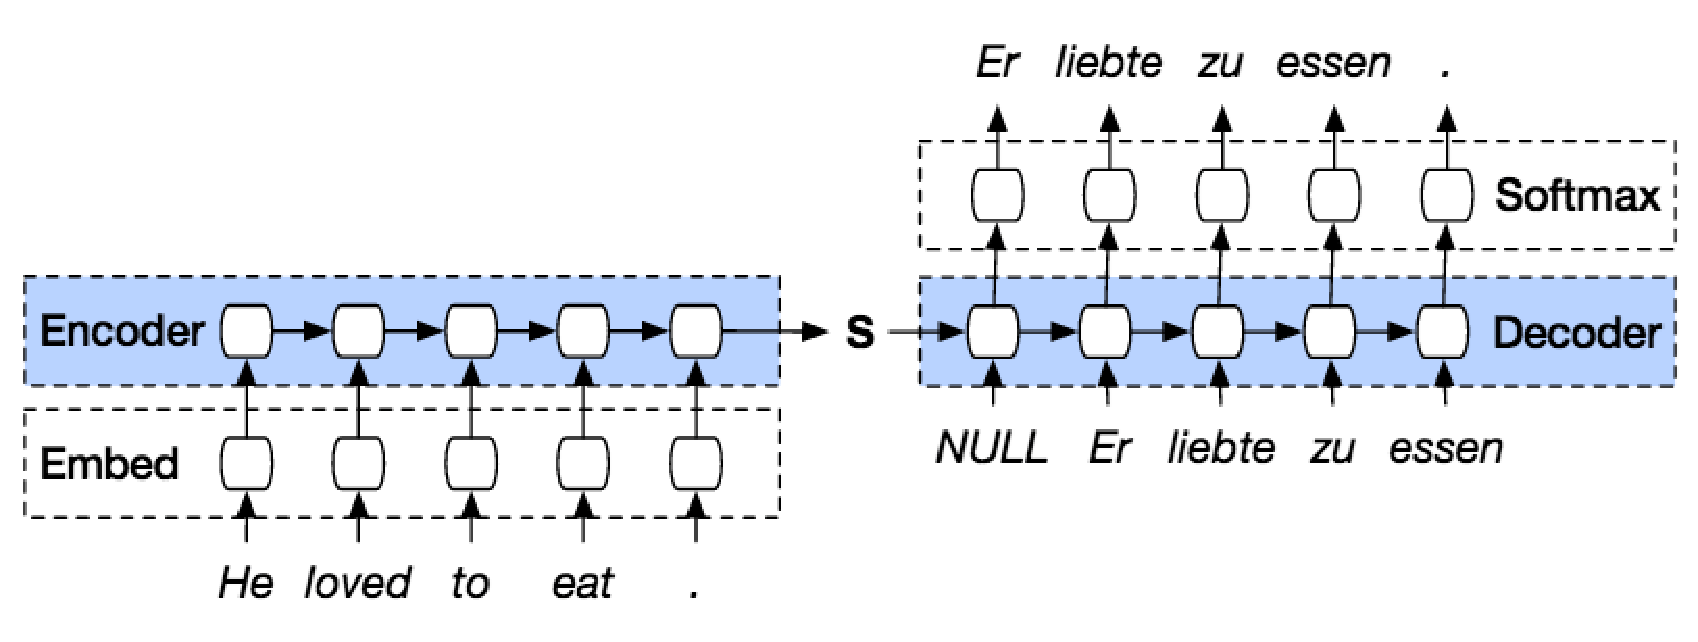
\includegraphics[width=8cm]{Figs/machine_translation.eps}
        \caption{Simple Machine Translation Model, \href{https://www.guru99.com/seq2seq-model.html} 
        {source}}
\end{figure}

\begin{itemize}
        \item We have discussed about Machine Translation models. We are familiar with some of their elements, namely, word embedding, encoder, decoder, S (context vector), and softmax. But, there is a missing part! The search strategy for inference.
        $$
        \Hat{y_T}, \Hat{y_{T-1}}, ..., \Hat{y_1} = \underset{\Tilde{y_T}, \Tilde{y_{T-1}}, ..., \Tilde{y_1}}{\mathbin{argmax}} P(\Tilde{y_T}, \Tilde{y_{T-1}}, ..., \Tilde{y_1}|S)
        $$
        \textbf{Notice:} $y_t$ is the corresponding word to time step t. 
\end{itemize}

}
%%%%%%%%%%%%%%%%%%%%%%%%%%%%%%%%%%%%%%%%%%%%%%%%%%%%%%%%%%%%%%%%%%%%%%%%%%%%%%%%%%%%%
\frame{\frametitle{Search Strategy}

\begin{itemize}
        \item \textbf{Exhaustive Search (Brute-force search)}
        \\
        Iterate over all possible combinations of $\Hat{y_t}, \Hat{y_{t-1}}, ..., \Hat{y_1}$.
        \vspace{3mm}
        \begin{itemize}
            \item T: Total Time Step (the number of decoder units)
            \vspace{3mm}
            \item V: Vocabulary Size (the number of possible words)
            \vspace{3mm}
            \item Time complexity: $O(V^T)$
            \vspace{3mm}
            \item So, it's not feasible.
        \end{itemize}
\end{itemize}


}
%%%%%%%%%%%%%%%%%%%%%%%%%%%%%%%%%%%%%%%%%%%%%%%%%%%%%%%%%%%%%%%%%%%%%%%%%%%%%%%%%%%%%
\frame{\frametitle{Search Strategy}
\begin{itemize}
        \item \textbf{Greedy Search}
        $$
        \mathbin{max} \, P(\Tilde{y_T}, \Tilde{y_{T-1}}, ..., \Tilde{y_1}|S) = 
        \mathbin{max} \prod_{t=1}^T P(y_t|y_{t-1}, y_{t-2}, ..., y_1, S)
        $$
        $$
        \mathbin{max} \prod_{t=1}^T P(y_t|y_{t-1}, y_{t-2}, ..., y_1, S) 
        \approx \prod_{t=1}^T \mathbin{max}\,P(y_t|y_{t-1}, y_{t-2}, ..., y_1, S) 
        $$
\end{itemize}

\begin{figure}[!h]
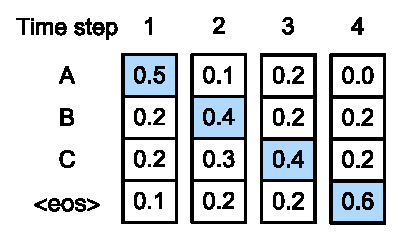
\includegraphics[width=4cm]{Figs/greedy2.eps}
        \caption{Greedy Search Example, \href{https://d2l.ai/chapter\_recurrent-modern/beam-search.html} 
        {source}}
\end{figure}
$$
P((A, B, C, eos)|S) = P(A|(), S) P(B|(A), S) P(C|(A, B), S) P(eos|(A, B, C), S)
$$ $$= 0.048$$

}
%%%%%%%%%%%%%%%%%%%%%%%%%%%%%%%%%%%%%%%%%%%%%%%%%%%%%%%%%%%%%%%%%%%%%%%%%%%%%%%%%%%%%
\frame{\frametitle{Search Strategy}
\begin{itemize}
        \item \textbf{Greedy Search}
        \vspace{3mm}
        \begin{itemize}
            \item Advantages
            \begin{enumerate}
                \item Time complexity: $O(TV)$
                \item Sometimes it's a good approximation
            \end{enumerate}
            \vspace{5mm}
            \item Disadvantages
            \begin{enumerate}
                \item It is somehow too naive. 
                \item It can be very inaccurate.
            \end{enumerate}

        \end{itemize}
\end{itemize}

\begin{figure}[!h]
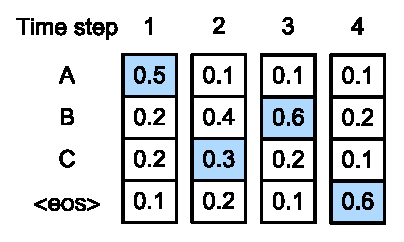
\includegraphics[width=4cm]{Figs/greedy.eps}
        \caption{Greedy Search Example, \href{https://d2l.ai/chapter\_recurrent-modern/beam-search.html} 
        {source}}
\end{figure}
$$
P((A, C, B, eos)|S) = P(A|(), S) P(C|(A), S) P(B|(A, C), S) P(eos|(A, C, B), S) 
$$ $$= 0.054$$

}
%%%%%%%%%%%%%%%%%%%%%%%%%%%%%%%%%%%%%%%%%%%%%%%%%%%%%%%%%%%%%%%%%%%%%%%%%%%%%%%%%%%%%
\frame{\frametitle{Beam Search}
\begin{itemize}
        \item \textbf{Beam Search}
        \\ It's something between the two previous methods.
        \begin{itemize}
            \item Keeping a number of candidates (beam width) instead of one in Greedy Search and all of the combinations in Exhaustive Search. 
        \end{itemize}
\end{itemize}

\begin{figure}[!h]
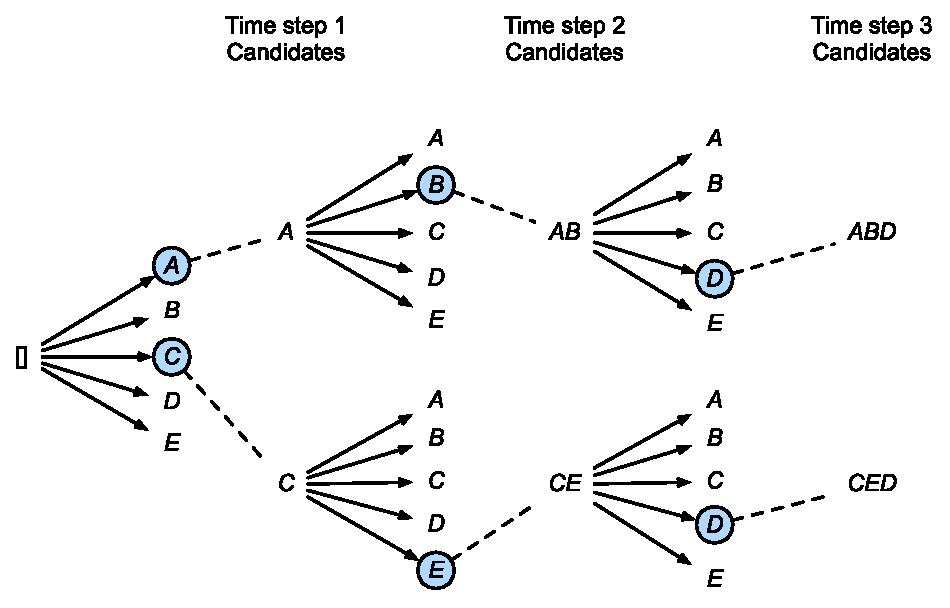
\includegraphics[width=7cm]{Figs/beam-search.eps}
        \caption{A Beam Search example in which beam width equals 2, \href{https://d2l.ai/chapter\_recurrent-modern/beam-search.html} 
        {source}}
\end{figure}

}
%%%%%%%%%%%%%%%%%%%%%%%%%%%%%%%%%%%%%%%%%%%%%%%%%%%%%%%%%%%%%%%%%%%%%%%%%%%%%%%%%%%%%
\frame{\frametitle{Beam Search}
\begin{itemize}
        \item \textbf{Beam Search}
        \\ It's something between the two previous methods.
        \begin{itemize}
            \item k: Beam width 
            \vspace{3mm}
            \item Time complexity: $O(\mathbin{log(k)kVT})$ (By using max heap in each time step)
        \end{itemize}
\end{itemize}

\begin{figure}[!h]
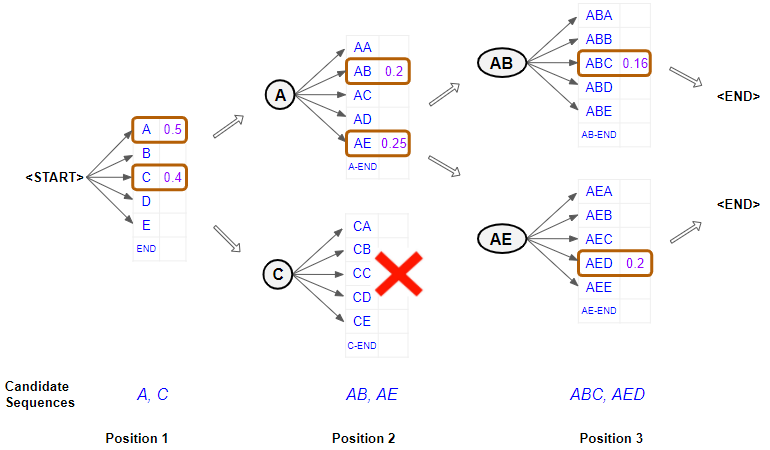
\includegraphics[width=7cm]{Figs/beam-search2.png}
        \caption{Another Beam Search example in which beam width equals 2, \href{https://towardsdatascience.com/foundations-of-nlp-explained-visually-beam-search-how-it-works-1586b9849a24} 
        {source}}
\end{figure}

}
%%%%%%%%%%%%%%%%%%%%%%%%%%%%%%%%%%%%%%%%%%%%%%%%%%%%%%%%%%%%%%%%%%%%%%%%%%%%%%%%%%%%%
%%%%%%%%

\frame{\frametitle{References}

\begin{itemize}

\item https://lilianweng.github.io/posts/2018-06-24-attention/
\vspace{3mm}
\item https://mmuratarat.github.io/2019-02-07/bptt-of-rnn
\vspace{3mm}
\item https://d2l.ai/chapter\_recurrent-modern/encoder-decoder.html
\vspace{3mm}
\item https://d2l.ai/chapter\_recurrent-modern/seq2seq.html
\vspace{3mm}
\item https://d2l.ai/chapter\_recurrent-modern/beam-search.html
\vspace{3mm}
\end{itemize}

}
%%%%%%%%%%%%%%%%%%%%%%%%%%%%%%%%%%%%%%%%%%%%%%%%%%%%%%%%%%%%%%%%%%%%%%%%%%%%%%%%%%%%%

\frametitle{Final Notes}
\centering
\vspace{50 pt}
\textbf{Thank You!}
\vspace{50pt}

\textbf{Any Question?}
%%%%%%%%%%%%%%%%%%%%%%%%%%%%%%%%%%%%%%%%%%
\end{document}